\title{Architectural Views}
\author{Richard Thomas \& Brae Webb}
\date{\week{1}}

\maketitle

\section{Introduction}

Understanding software is hard.
It is often claimed that reading code is harder than writing code\footnote{Though evidence suggests that an ability to read and reason 
about code is necessary to learn how to program well \cite{lister-tracing-explaining-writing} \cite{lister-neo-piagetian}.}.
This principle is used to explain a programmer's innate desire to constantly rewrite their code from scratch.
If software is hard to understand, then understanding software architecture from the detail of the code is near impossible.
Fortunately, architects have developed a number of techniques to manage this complexity.

A software architecture consists of many dimensions.
Programming languages, communication protocols, the operating systems and hardware used, virtualisation used,
and the code itself are a subset of the many dimensions which comprise a software architecture.
Asking a programmer's monkey brain to understand, communicate, or document every dimension at once is needlessly cruel.
This is where architectural views come in.

Architectural views, or architectural projections, are a representation of one or more related aspects of a software architecture.
Views allow us to focus on a particular slice of our multi-dimensional software architecture, ignoring other irrelevant slices.
For example, if we are interested in applying a security patch to our software then we are only interested in the view
which tells us which software packages are used on each host machine.

The successful implementation of any architecture relies on the ability for the architectural views
to be disseminated, understood, and implemented.
For some organisations, the software is simple enough, or the team small enough, that the design
can be communicated through word of mouth.
As software becomes increasingly complex and developers number in the thousands,
it is critical for design to be communicated as effectively as possible.
In addition to facilitating communication,
architectural views also enable architectural policies to be designed and implemented.


\section{C4 Model}
Simon Brown's C4 model provides a set of abstractions that describe the static structure of the software architecture \cite{brown2022c4}.
The C4 model uses these abstractions in a hierarchical set of diagrams, each leading to finer levels of detail.
The hierarchical structure is based on the idea that a software system is composed of containers, which are implemented by components, that are built using code.
\begin{description}
    \item[Software System] Something that delivers functional value to its users (human or other systems).
    \item[Containers] Deployable `block' of code or data that provides behaviour as part of the software system.
    \item[Components] Encapsulate a group of related functionality, usually hidden behind a published interface.
    \item[Code] Elements built from programming language constructs, e.g. classes, interfaces, functions, ....
\end{description}

\begin{figure}[h]
    \centering
    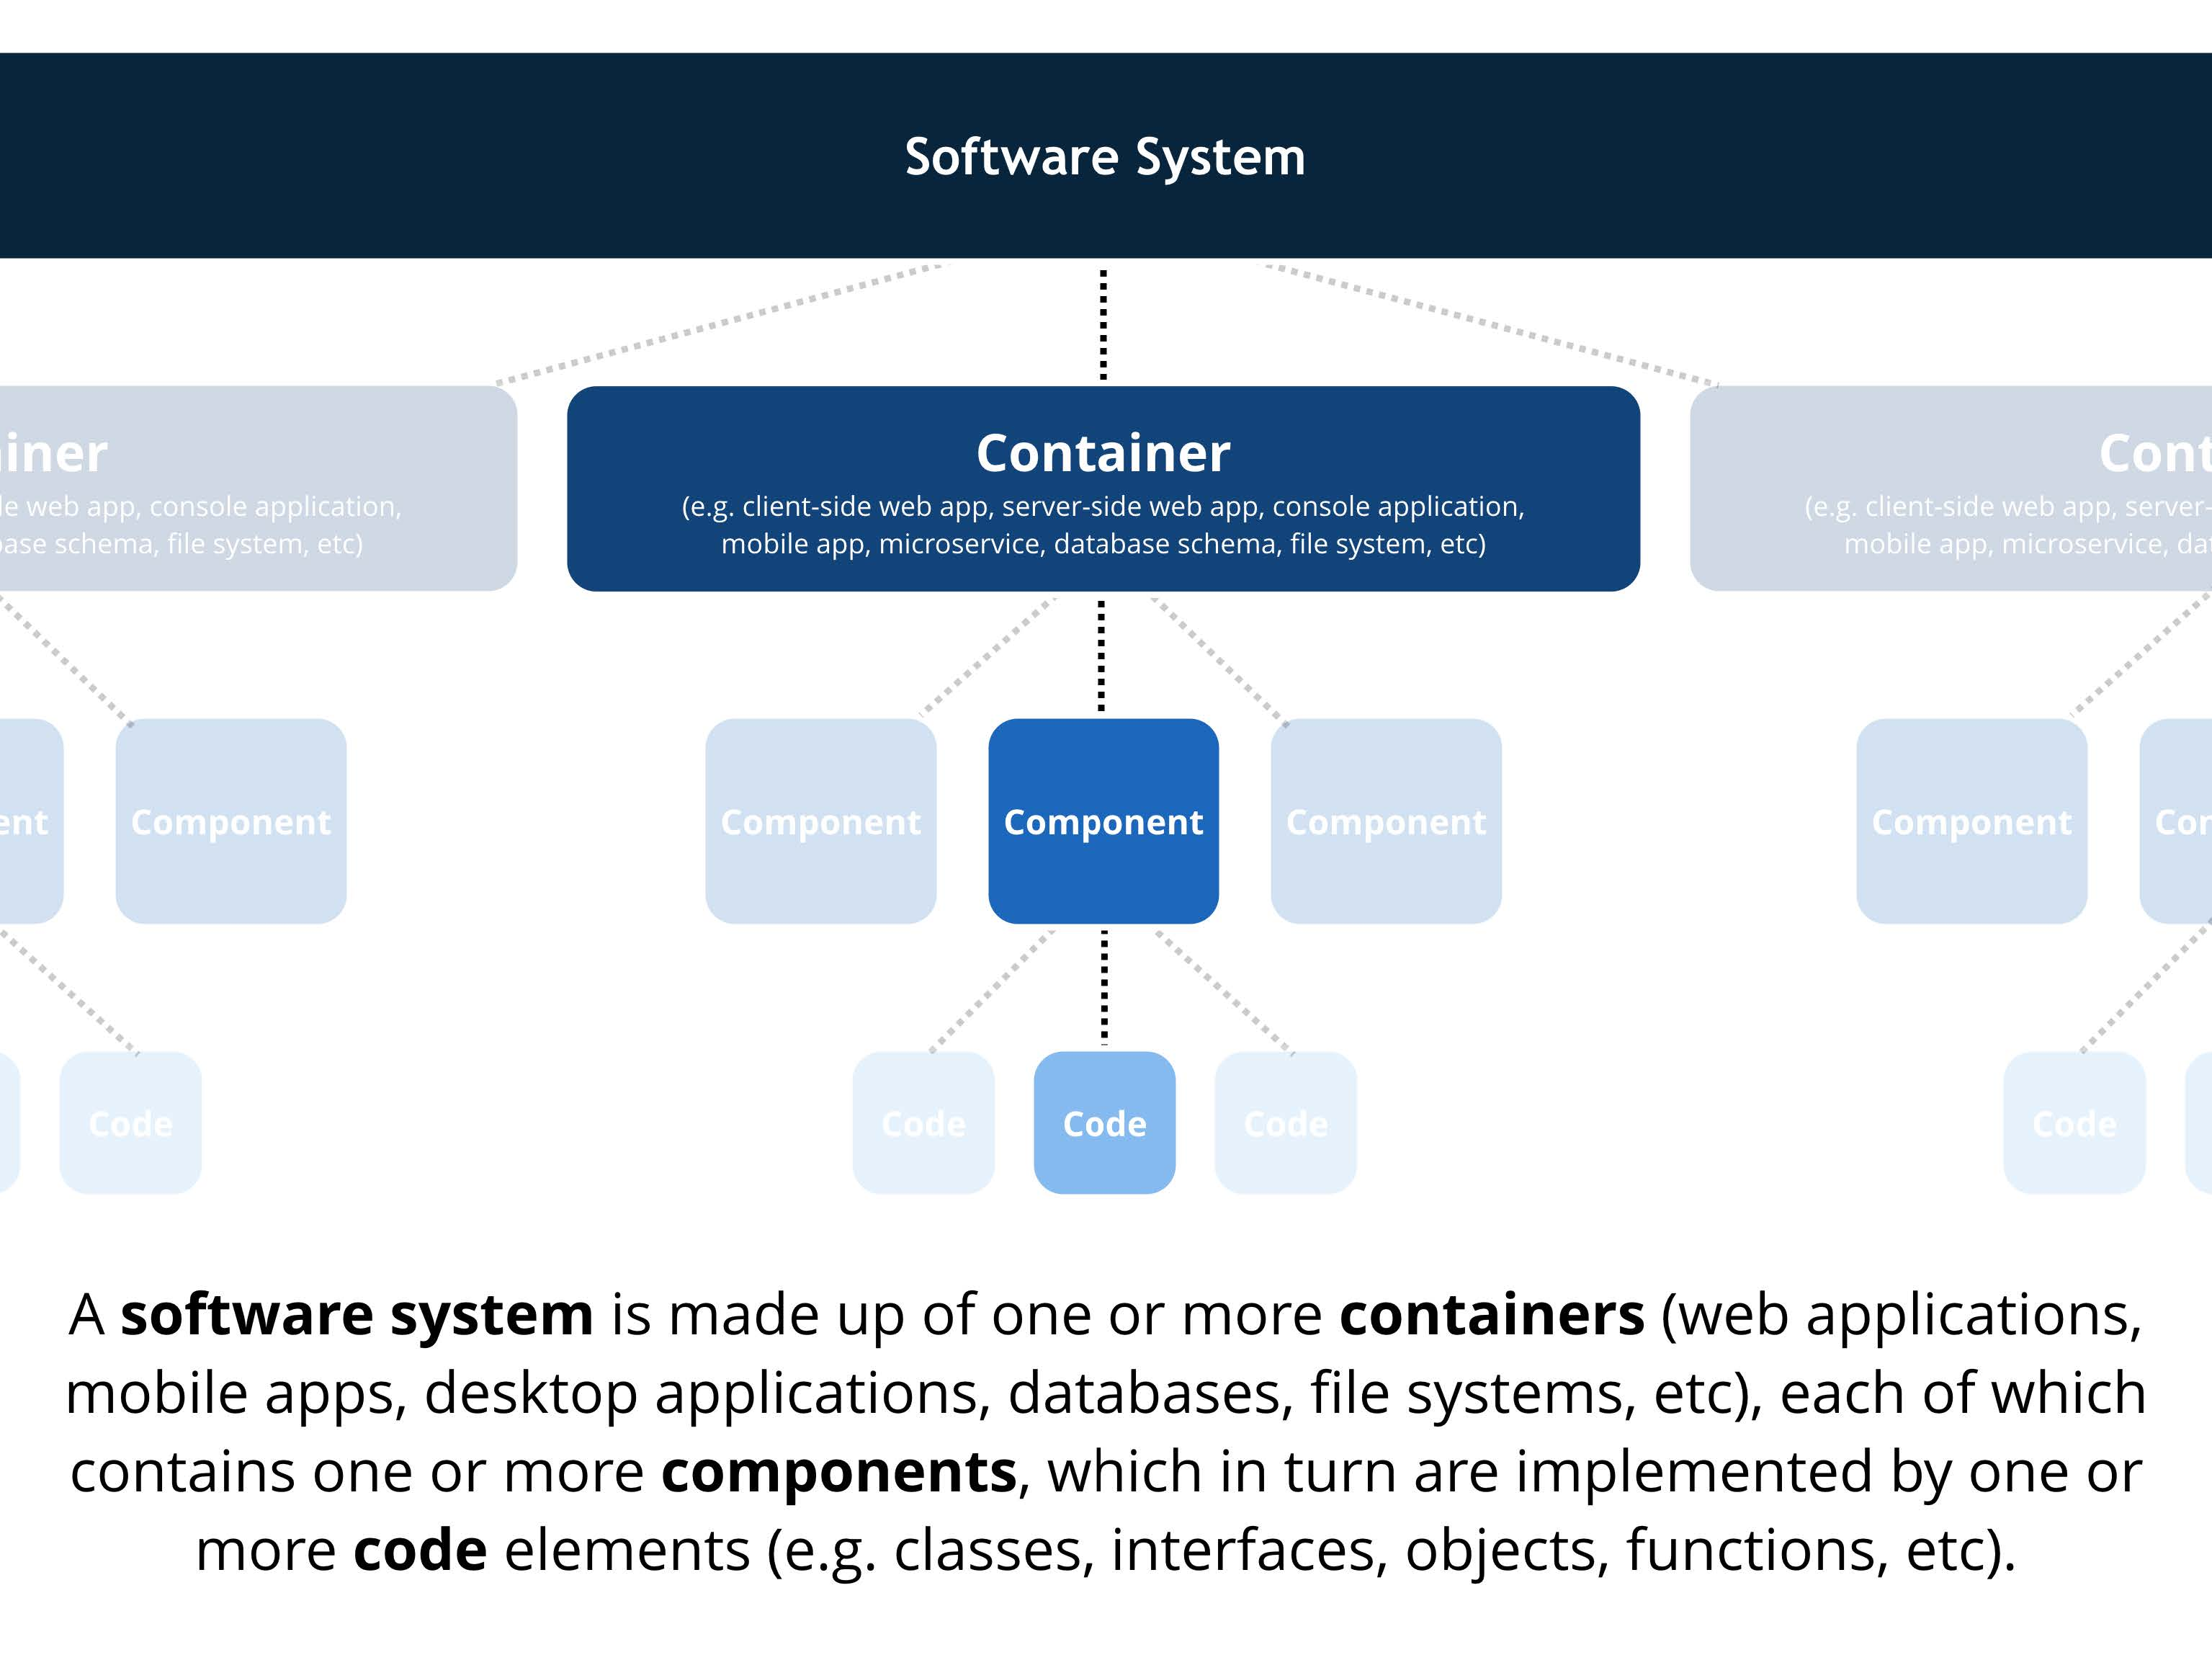
\includegraphics[trim=0 8 0 5,clip,width=0.8\textwidth]{images/c4_terminology.jpg}
    \caption{Levels within the C4 model (figure 2.1 from \cite{brown2022c4}).}
    \label{fig:c4terms}
\end{figure}

\noindent
The C4 model does not explicitly identify different architectural views,
but views are implicit in the types of diagrams produced to describe an architecture.

\newpage
The static \emph{structural} view of software architecture is described through four levels of abstraction.
Each level providing detail about parts of the previous level.
\begin{description}
    \item[Context] How the software system fits into the broader context around it.
    \item[Containers] How the containers are connected to deliver system functionality.
    \item[Components] How the components are structured to implement a container's behaviour.
    \item[Code] How the code is structured to implement a component.
\end{description}

The \emph{behavioural} view is described via a dynamic diagram that describes how
containers and components interact to deliver system features.

The \emph{infrastructure} view is described by a deployment diagram that describes how
executable containers, software systems, and other infrastructure services are
deployed on computing platforms to instantiate the system.


\section{Sahara eCommerce Example}\label{sec:storeExample}
Sahara\footnote{Yes, that is intentionally a \textit{dry} joke.} eCommerce is an ambitious company who's prime business unit is an on-line store selling a wide range of products.
Sahara provides both web and mobile applications to deliver the shopping experience to customers.

\subsection{Architecturally Significant Requirements}\label{sec:storeReq}
\emph{Architecturally significant requirements} (ASR) are functional or non-functional requirements,
or constraints or principles, which influence the design of the system architecture.
The structure of a software architecture has to be designed to ensure that the ASRs can be delivered.

Not all requirements for a system will be architecturally significant, but those that are need to be identified.
Once ASRs are identified, an architecture needs to be designed to deliver them.
This may require some research, and experimentation with prototypes, to determine which options are appropriate.
Tests should be designed to verify that the architecture is delivering the ASRs.
Ideally, these should be part of an automated test suite.
This may not be possible for all tests.
Regardless, the ASR tests should be executed frequently during development to provide assurance that the system will deliver the ASRs.

Inevitably, some ASRs will be discovered later in the project.
The existing architecture will need to be evaluated to determine if it can deliver the new ASRs.
If it can, new tests need to be added to the ASR test suite to verify delivery of the new ASRs.
If the architecture is no longer suitable due to the new ASRs,
a major redesign needs to be done to create a new, more suitable, architecture.

The architecturally significant requirements for the Sahara eCommerce system are:
\begin{itemize}
    \item Customers can start shopping on one device and continue on another device.
             (e.g. Add a product to their shopping cart while browsing on their computer when they are bored at school.
              Checkout their shopping cart from their mobile phone on their way home on the bus.)
    \item The system must be scalable. It must cater for peaks in demand (e.g. Cyber Monday and Singles Day).
             It must cater for an unknown distribution of customers accessing the on-line store through web or mobile applications.
    \item The system must be robust. The system must continue to operate if a server fails.
             It must be able to recover quickly from sub-system failures.
    \item The system must have high availability.
             Target availability is ``four nines''\footnote{A number of nines (e.g. four nines)
             is a common way to measure availability. It represents the percentage of time the system is ``up''.
             Four nines means the system is available 99.99\% of the time, or it is not available for less than one hour per year.}
            up time.
\end{itemize}
\noindent
The following sections will describe the physical and software architecture for this system, and demonstrate how it delivers these ASRs.

\subsection{System Context}
The system context provides the `big picture' perspective of the software system.
It describes the key purpose of the system, who uses it, and with which other systems it interacts.
The context diagram is usually a simple block diagram.
The software system being designed typically sits in the centre of the diagram surrounded by users and other systems.
The intent is to set the context for thinking about the software system's architecture.
It can also be used to communicate basic structural ideas to non-technical stakeholders.
Figure \ref{fig:c4_context} is a context diagram for the Sahara eCommerce system.
The overall eCommerce system is delivered through two interacting software systems,
the on-line store and the data mining service.

\begin{figure}[h]
  {
    \centering
    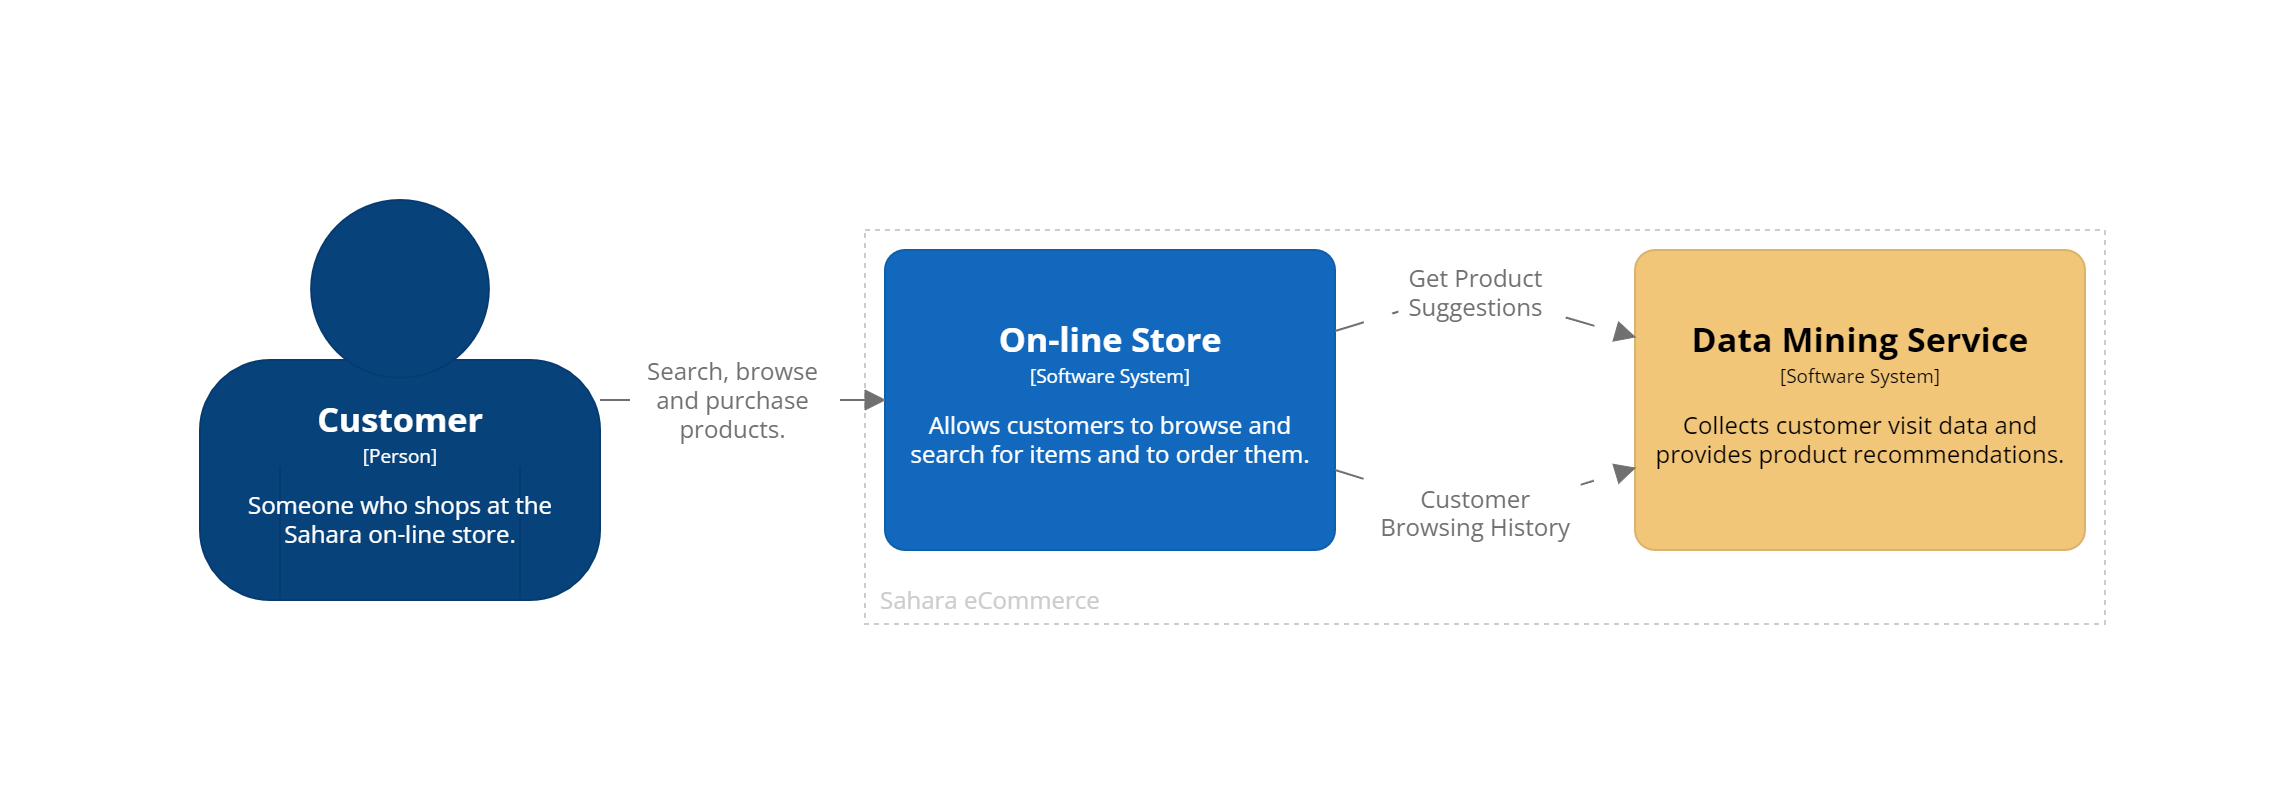
\includegraphics[trim=195 195 198 195,clip,width=\textwidth]{images/c4/context_diagram.png}
    \caption{Context diagram for the Saraha eCommerce on-line store.}
    \label{fig:c4_context}
  }
\end{figure}

\noindent
Figure \ref{fig:c4_context_key} is the key to help interpret the context diagram.
A key is important for C4 diagrams, as they have a fairly informal syntax and specification.

\begin{figure}[h]
  {
    \centering
    \begin{adjustwidth}{-7.5mm}{-7.5mm}
        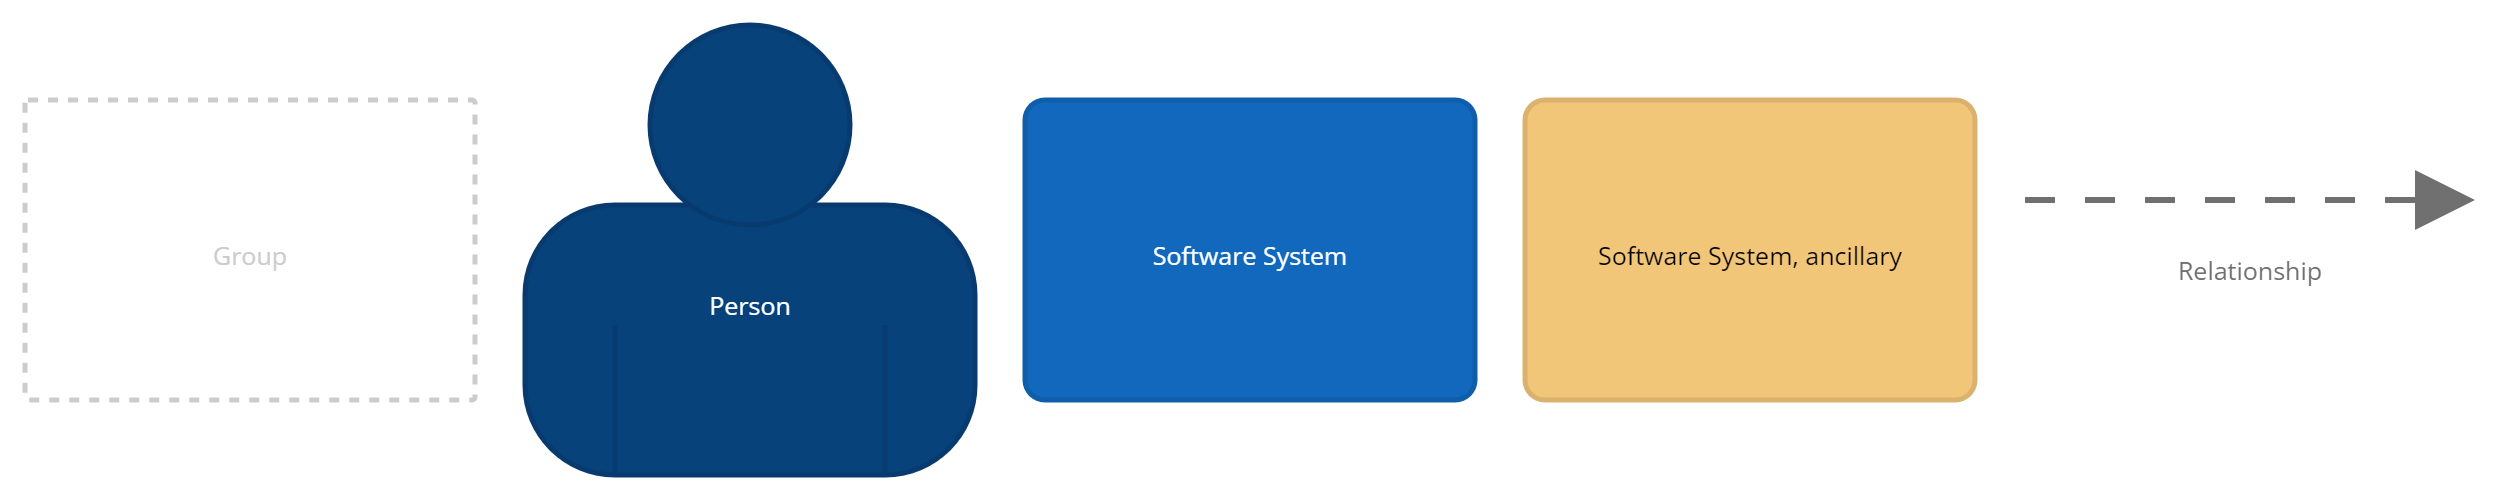
\includegraphics[trim=20 15 20 18,clip,width=0.95\paperwidth]{images/c4/context_diagram-key.png}
    \end{adjustwidth}
    \caption{Context diagram key.}
    \label{fig:c4_context_key}
  }
\end{figure}

\noindent
The context diagram situates the on-line store software system in the environment in which it will be used.
There are customers who shop at the on-line store, which is part of Sahara eCommerce's software ecosystem.
The on-line store uses a data mining service that is also implemented by the company.
The two key relationships between the on-line store and the data mining service are 
that the on-line store sends customer browsing data to the service,
and that the on-line store requests the data mining service to recommend products for a customer.

In C4, arrows are used to indicate the main direction of the relationship, not the flow of data.
So, in this example, the arrow points from the on-line store to the data mining service as it is the store that manages the communication.

\subsection{Containers}
Container diagrams provide an overview of the software architecture.
They describe the main structure of the software system and the technologies selected to implement these aspects of the system.
Containers are `blocks' of code that can be independently deployed and executed.
Examples of containers are web or mobile applications, databases, message buses, ....
It is important to note that containers may be deployed on the same computing infrastructure or on different devices.

Container diagrams focus on the connections between containers and, to an extent, how they communicate.
They do not explicitly show computing infrastructure.
Decisions about how containers are connected and communicate have major implications for how the components and code will be designed and deployed.
Figure~\ref{fig:c4_container_store} is a container diagram for the on-line store.
For simplicity, containers managing load balancing and fail-over are not shown in this example.

To provide a link to the context diagram, a container diagram usually shows which containers communicate with which external elements.
The text inside the square brackets in a container, and on a relationship, indicates the technology used to implement that container or relationship.

\begin{figure}[h!]
    \centering
    \begin{adjustwidth}{-9mm}{-9mm}
        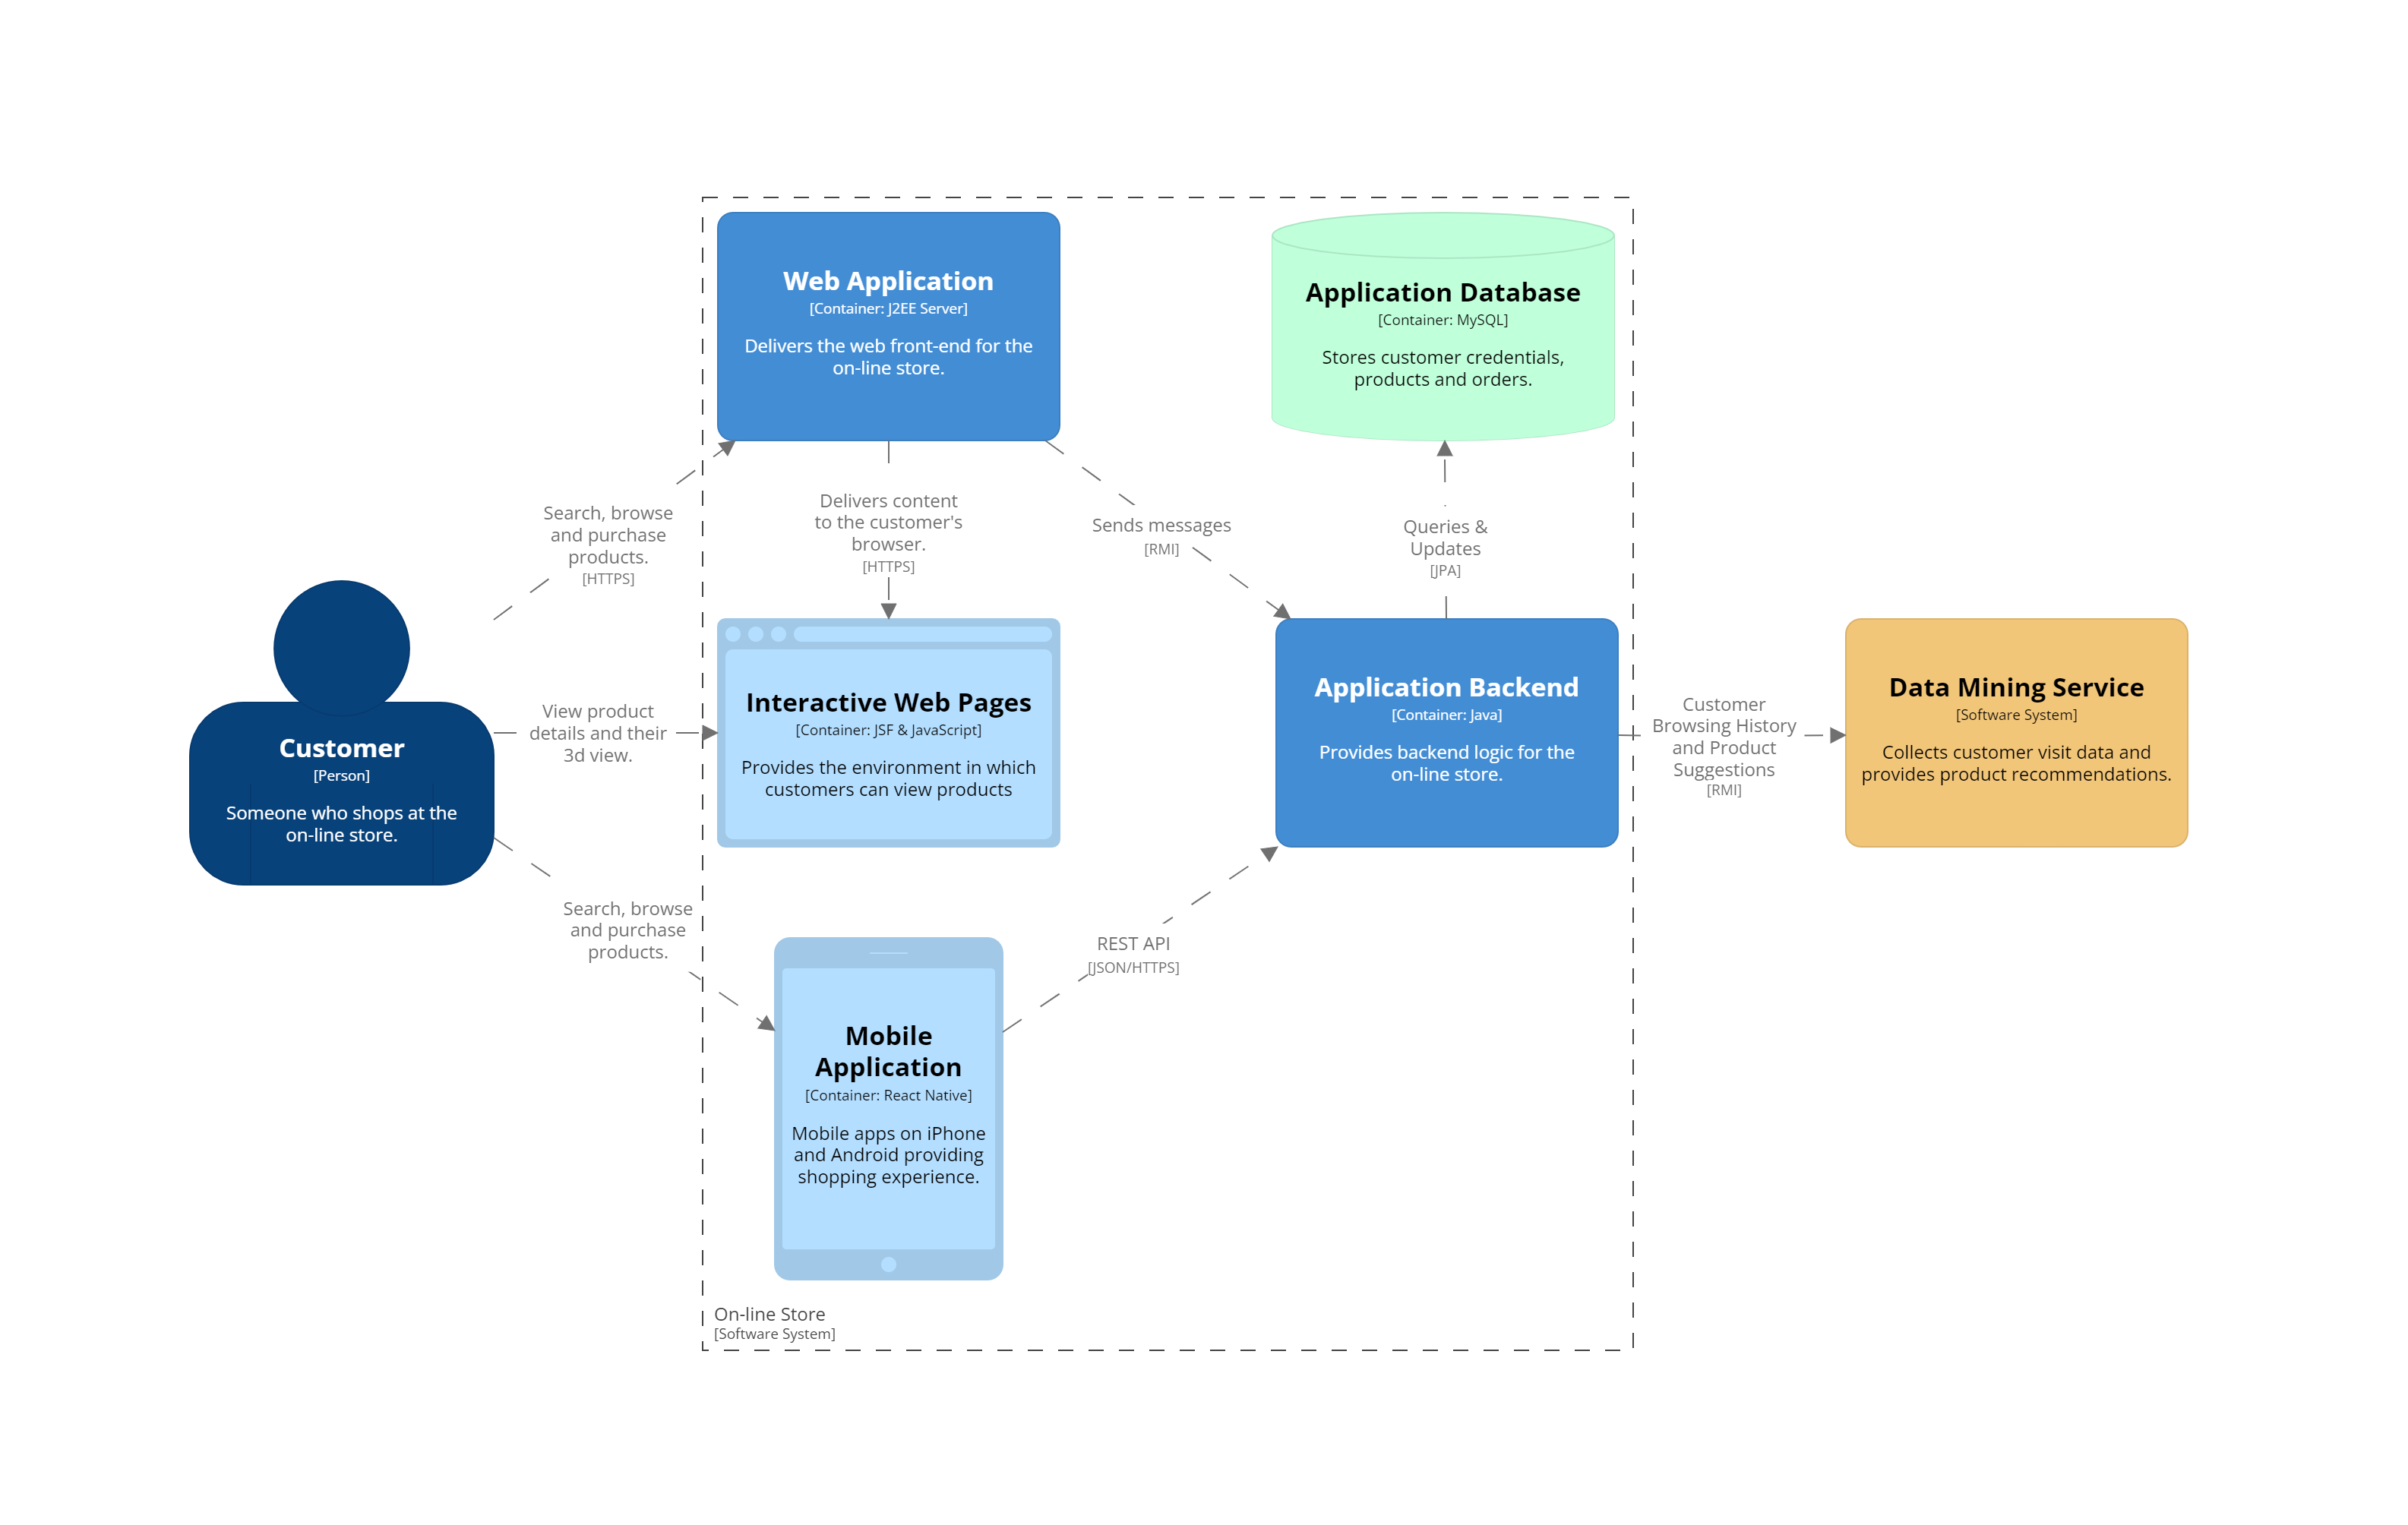
\includegraphics[trim=195 190 200 185,clip,width=0.96\paperwidth]{images/c4/store_container_diagram.png}
    \end{adjustwidth}
    \caption{Container diagram for the on-line store software system.}
    \label{fig:c4_container_store}
\end{figure}

Customers access the on-line store through either web or mobile applications.
The \texttt{Web Application} and \texttt{Interactive Web Pages} containers indicate
that the web application's behaviour is delivered by two different specialised containers.
The \texttt{Web Application} container indicates that it runs in a 
\href{https://jakarta.ee/}{J2EE}\footnote{Jakarta Enterprise Edition [\url{https://jakarta.ee/}]} server.
This implements the presentation layer of the web application in Java.
It handles browser requests from customers, using the HTTPS protocol over the Internet.

The \texttt{Interactive Web Pages} are
\href{https://jakarta.ee/specifications/faces/}{JSF}\footnote{Jakarta Faces [\url{https://jakarta.ee/specifications/faces/}]}
pages and JavaScript code that implement more sophisticated user interactions on web pages.
These run within the users' browsers.

The \texttt{Web Application} container uses
\href{https://www.oracle.com/java/technologies/jpl1-remote-method-invocation.html}{RMI}%
\footnote{Remote Method Invocation [\url{https://www.oracle.com/java/technologies/jpl1-remote-method-invocation.html}} 
to invoke functional behaviour in the \texttt{Application Backend} container.
It provides the shared logic of the on-line store.
This supports implementing the functional requirement that a customer can start shopping on one device and continue on another.

The mobile application communicates with the application backend via a
\link{REST API}{https://www.ibm.com/topics/rest-apis}.
The application backend uses \href{https://jakarta.ee/specifications/persistence/}
{JPA}\footnote{Jakarta Persistence API [\url{https://jakarta.ee/specifications/persistence/}]}
to manage persistent data in the application's database.
The application backend uses RMI to communicate with the data mining service,
sending customer browsing and search history to be used for data mining
and receiving product suggestions to present to customers.

While a container diagram does not explicitly show computing infrastructure,
some of it can be implied by the types of containers in the diagram.
Clearly, the mobile app and the code running in the interactive web pages
have to be separate computing platforms to the rest of the on-line store's software system.

\begin{figure}[h!]
    \centering
    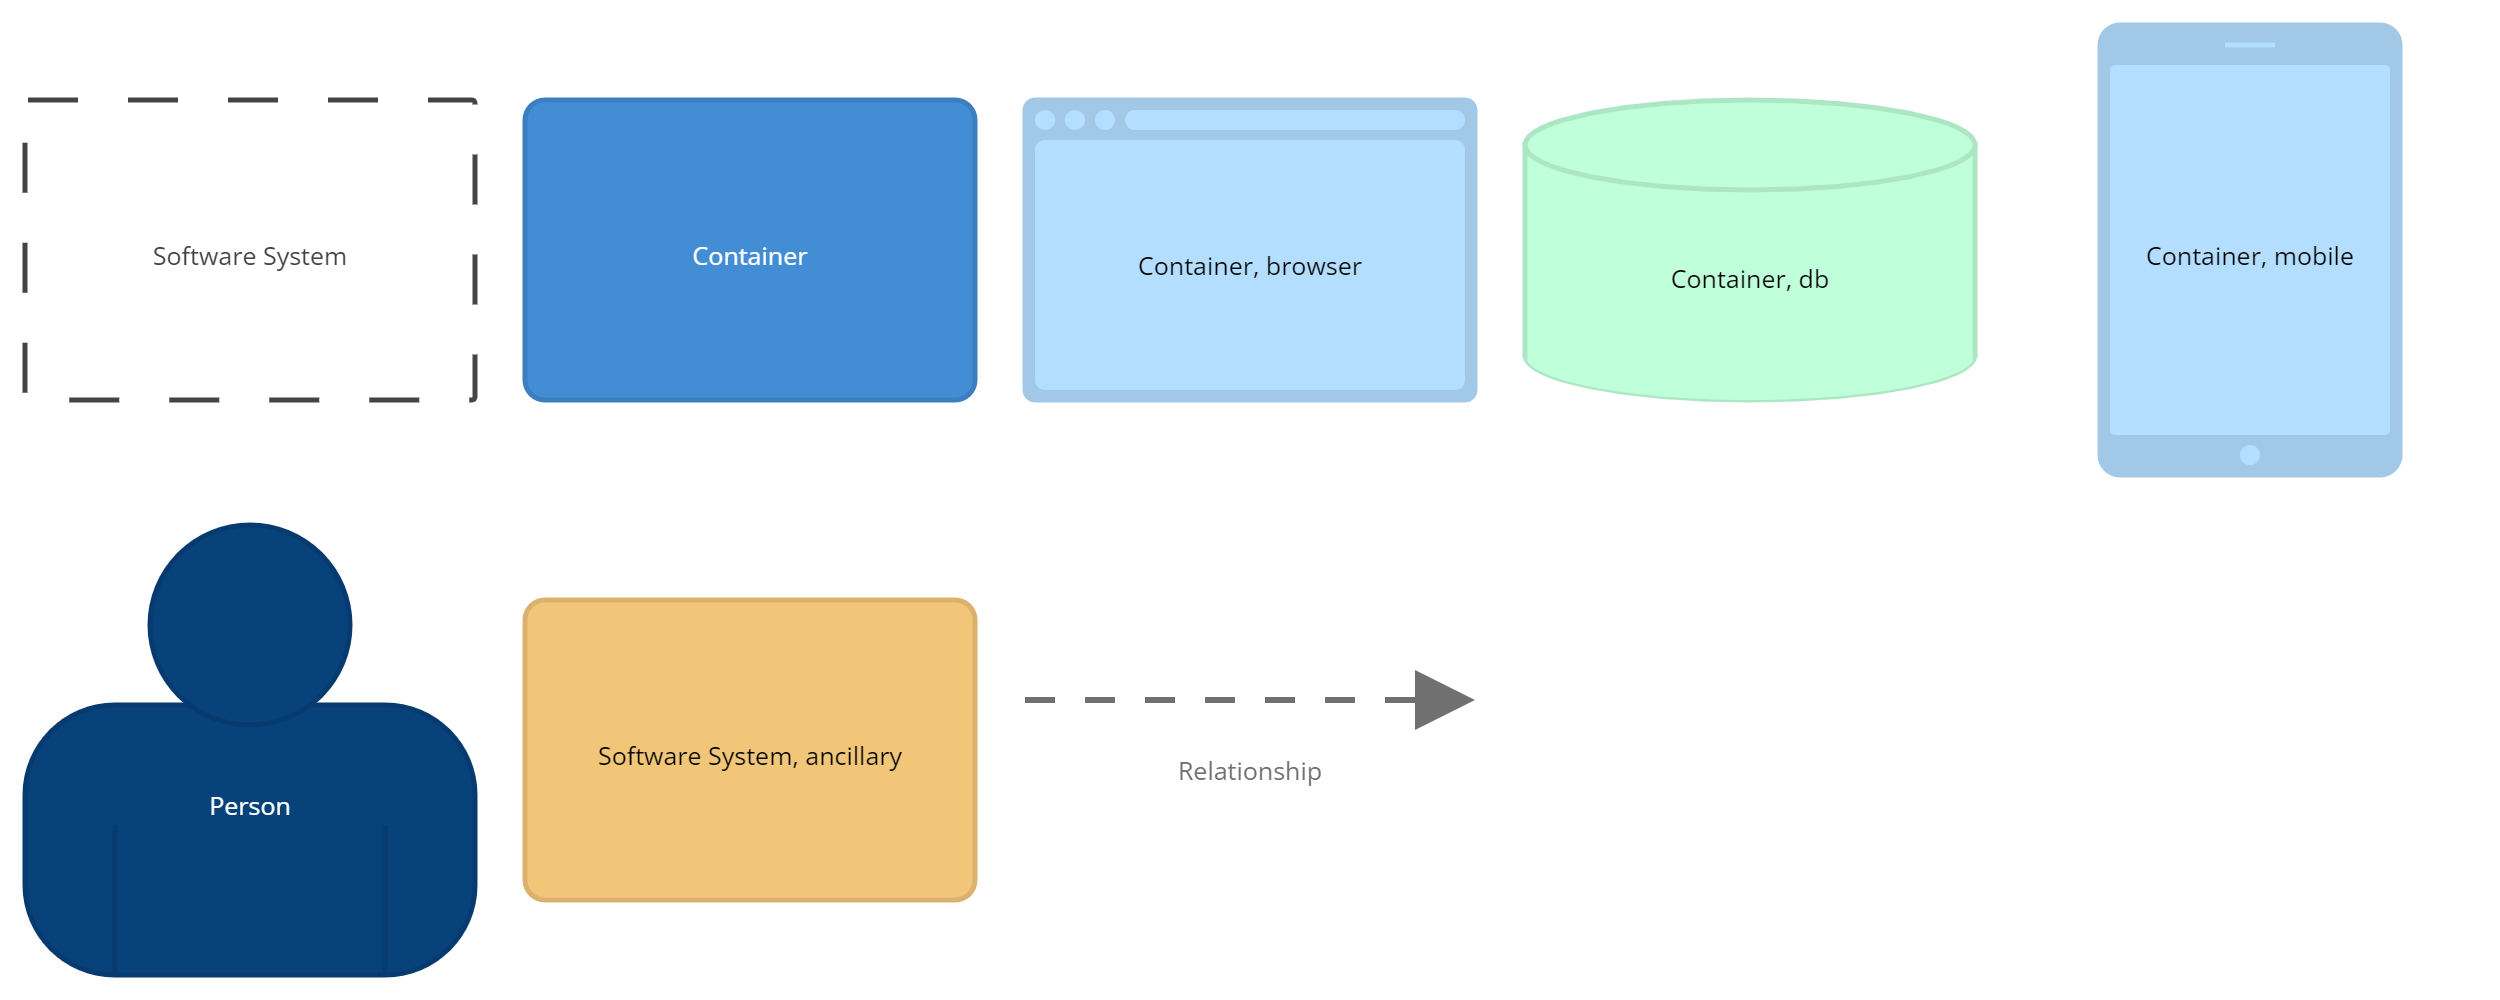
\includegraphics[trim=22 21 98 26,clip,width=\textwidth]{images/c4/container_diagram-key.png}
    \caption{Container diagram key.}
    \label{fig:c4_container_key}
\end{figure}

Colours and icons can be used to provide further information in the diagrams.
The diagram key in figure~\ref{fig:c4_container_key} explains the purpose of each icon and colour.

The data mining service software system (figure \ref{fig:c4_container_datamining}) has three main containers.

\texttt{Data Mining Interface} provides the interface used to interact with the data mining service.
It accepts data to store for future data mining.
It returns suggestions based on requests from external systems, such as the on-line store.

\texttt{Data Mining Process} performs the data mining logic.

\texttt{Data Warehouse} stores the data and provides an SQL-based query system to manipulate the data.
The data mining interface and process containers use
\href{https://docs.oracle.com/javase/tutorial/jdbc/basics/index.html}{JDBC}\footnote{Java DataBase Connectivity [\url{https://docs.oracle.com/javase/tutorial/jdbc/basics/index.html}]}
to work with the data in the data warehouse.

\begin{center}
    \begin{adjustwidth}{-5mm}{-5mm}
        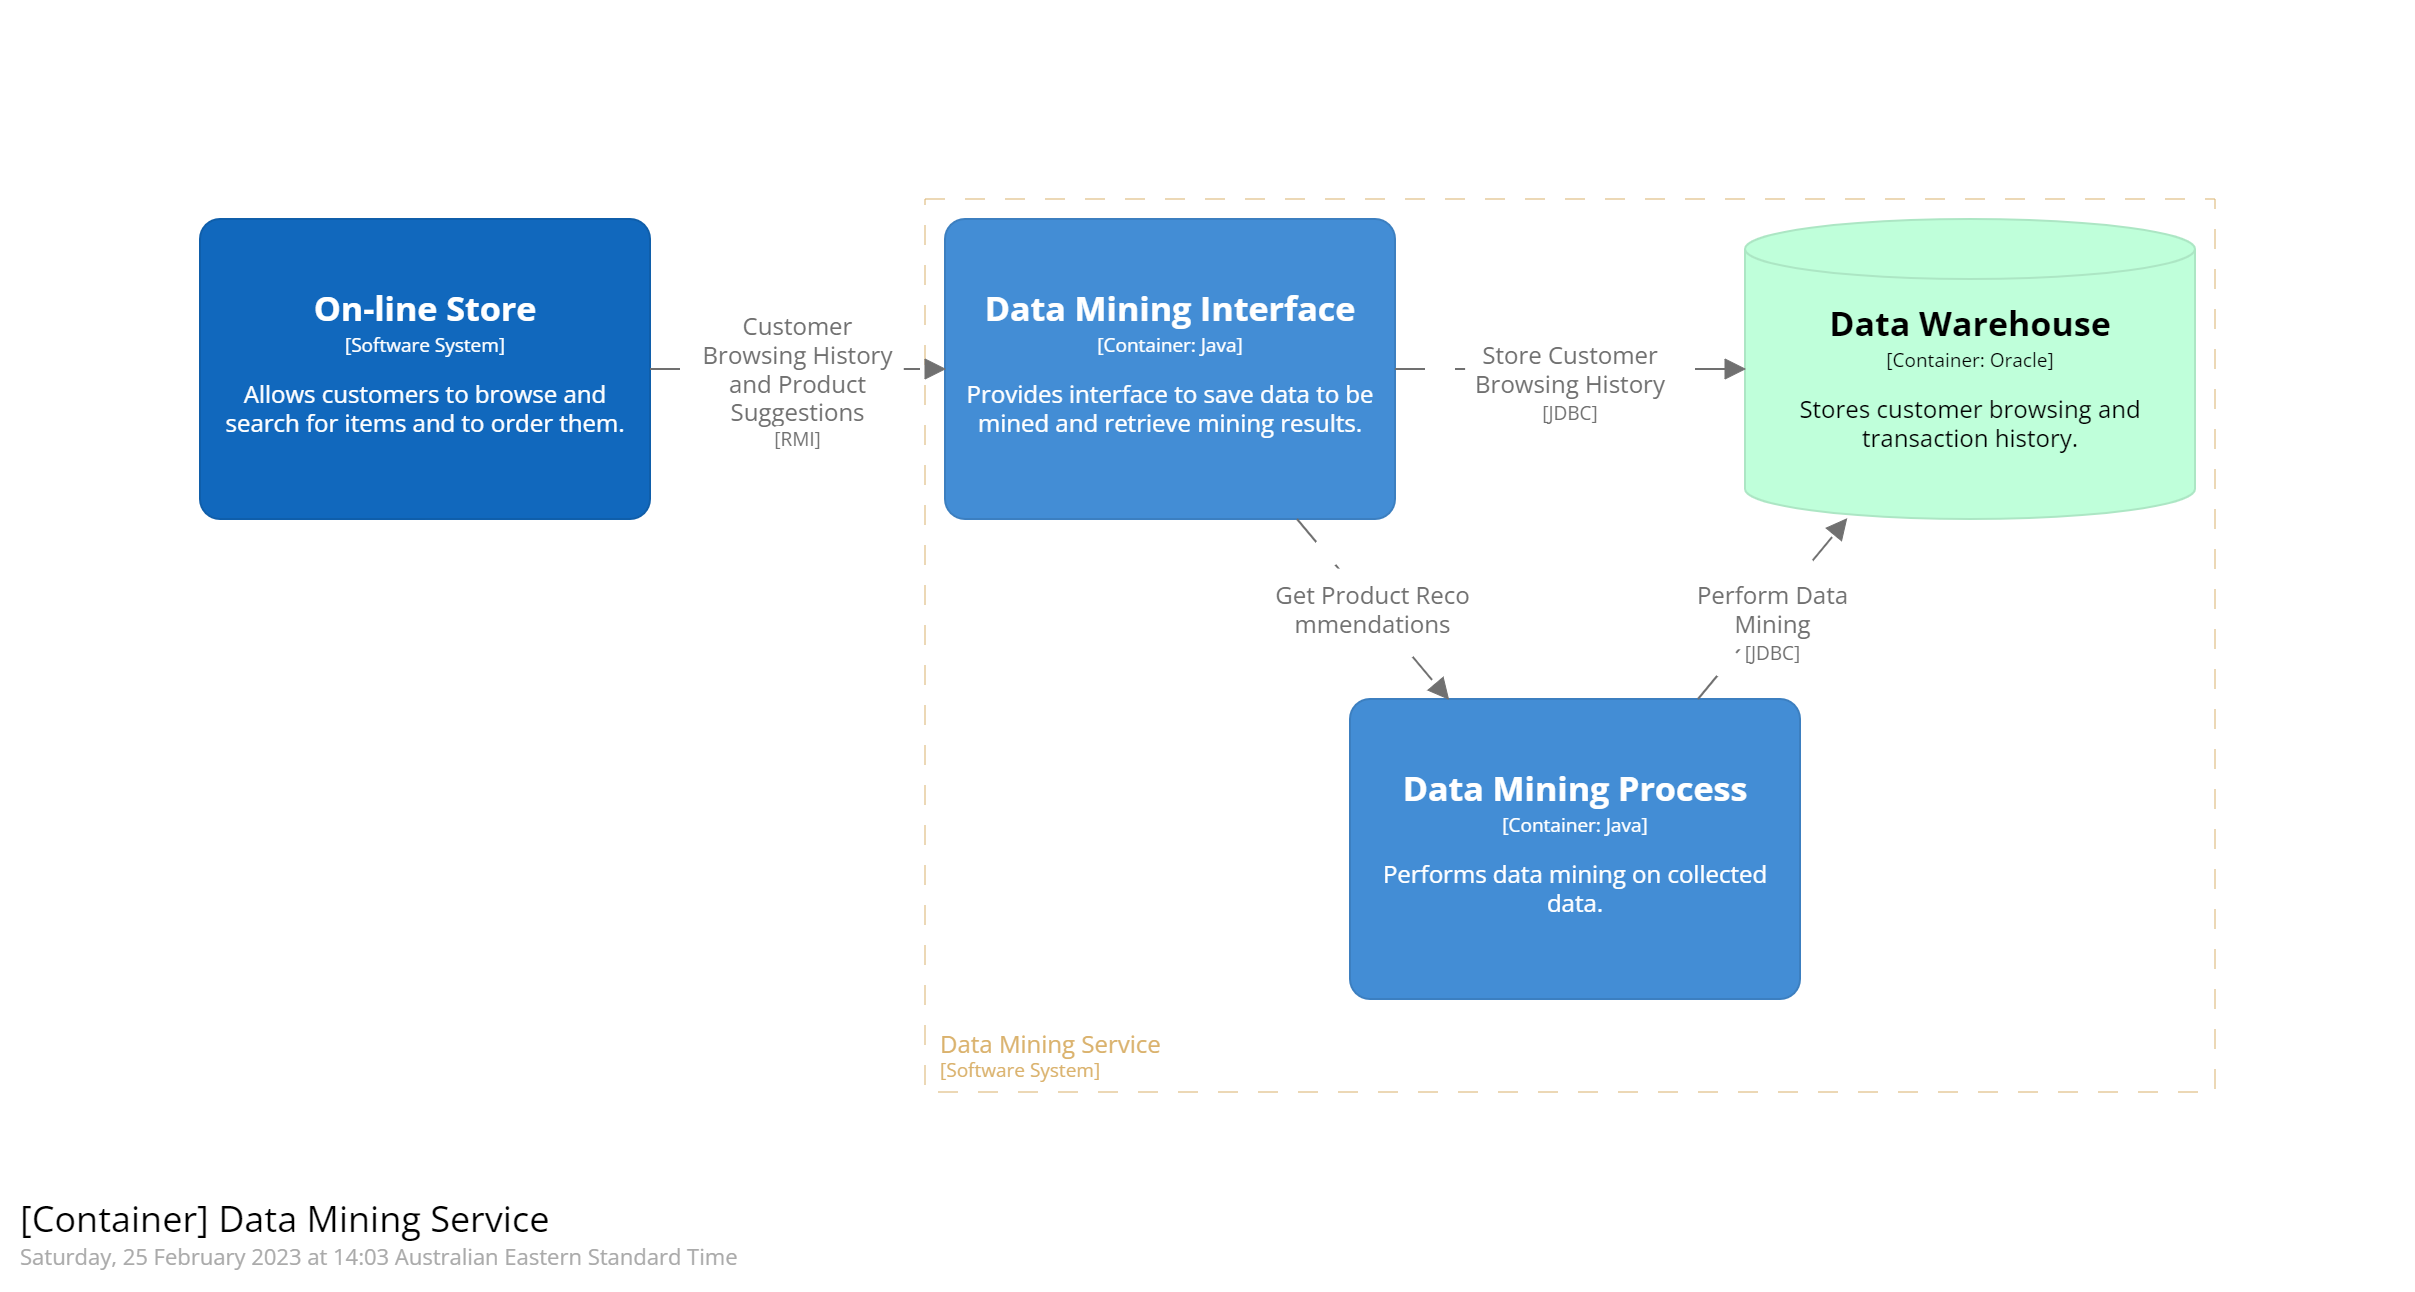
\includegraphics[trim=185 185 185 185,clip,width=0.92\paperwidth]{images/c4/datamining_container_diagram.png}
    \end{adjustwidth}
    \captionof{figure}{Container diagram for the data mining service software system.}
    \label{fig:c4_container_datamining}
\end{center}

\subsection{Components}
Component diagrams describe the major parts of containers and how they are connected.
Components should describe their important responsibilities and the technology used to implement them
(e.g. using React to implement a web frontend component).
Like a container diagram, a component diagram can include elements from higher level diagrams
to provide context of how the components interact with elements outside of the container.

\begin{figure}[h!]
    \centering
    \begin{adjustwidth}{-9mm}{-9mm}
        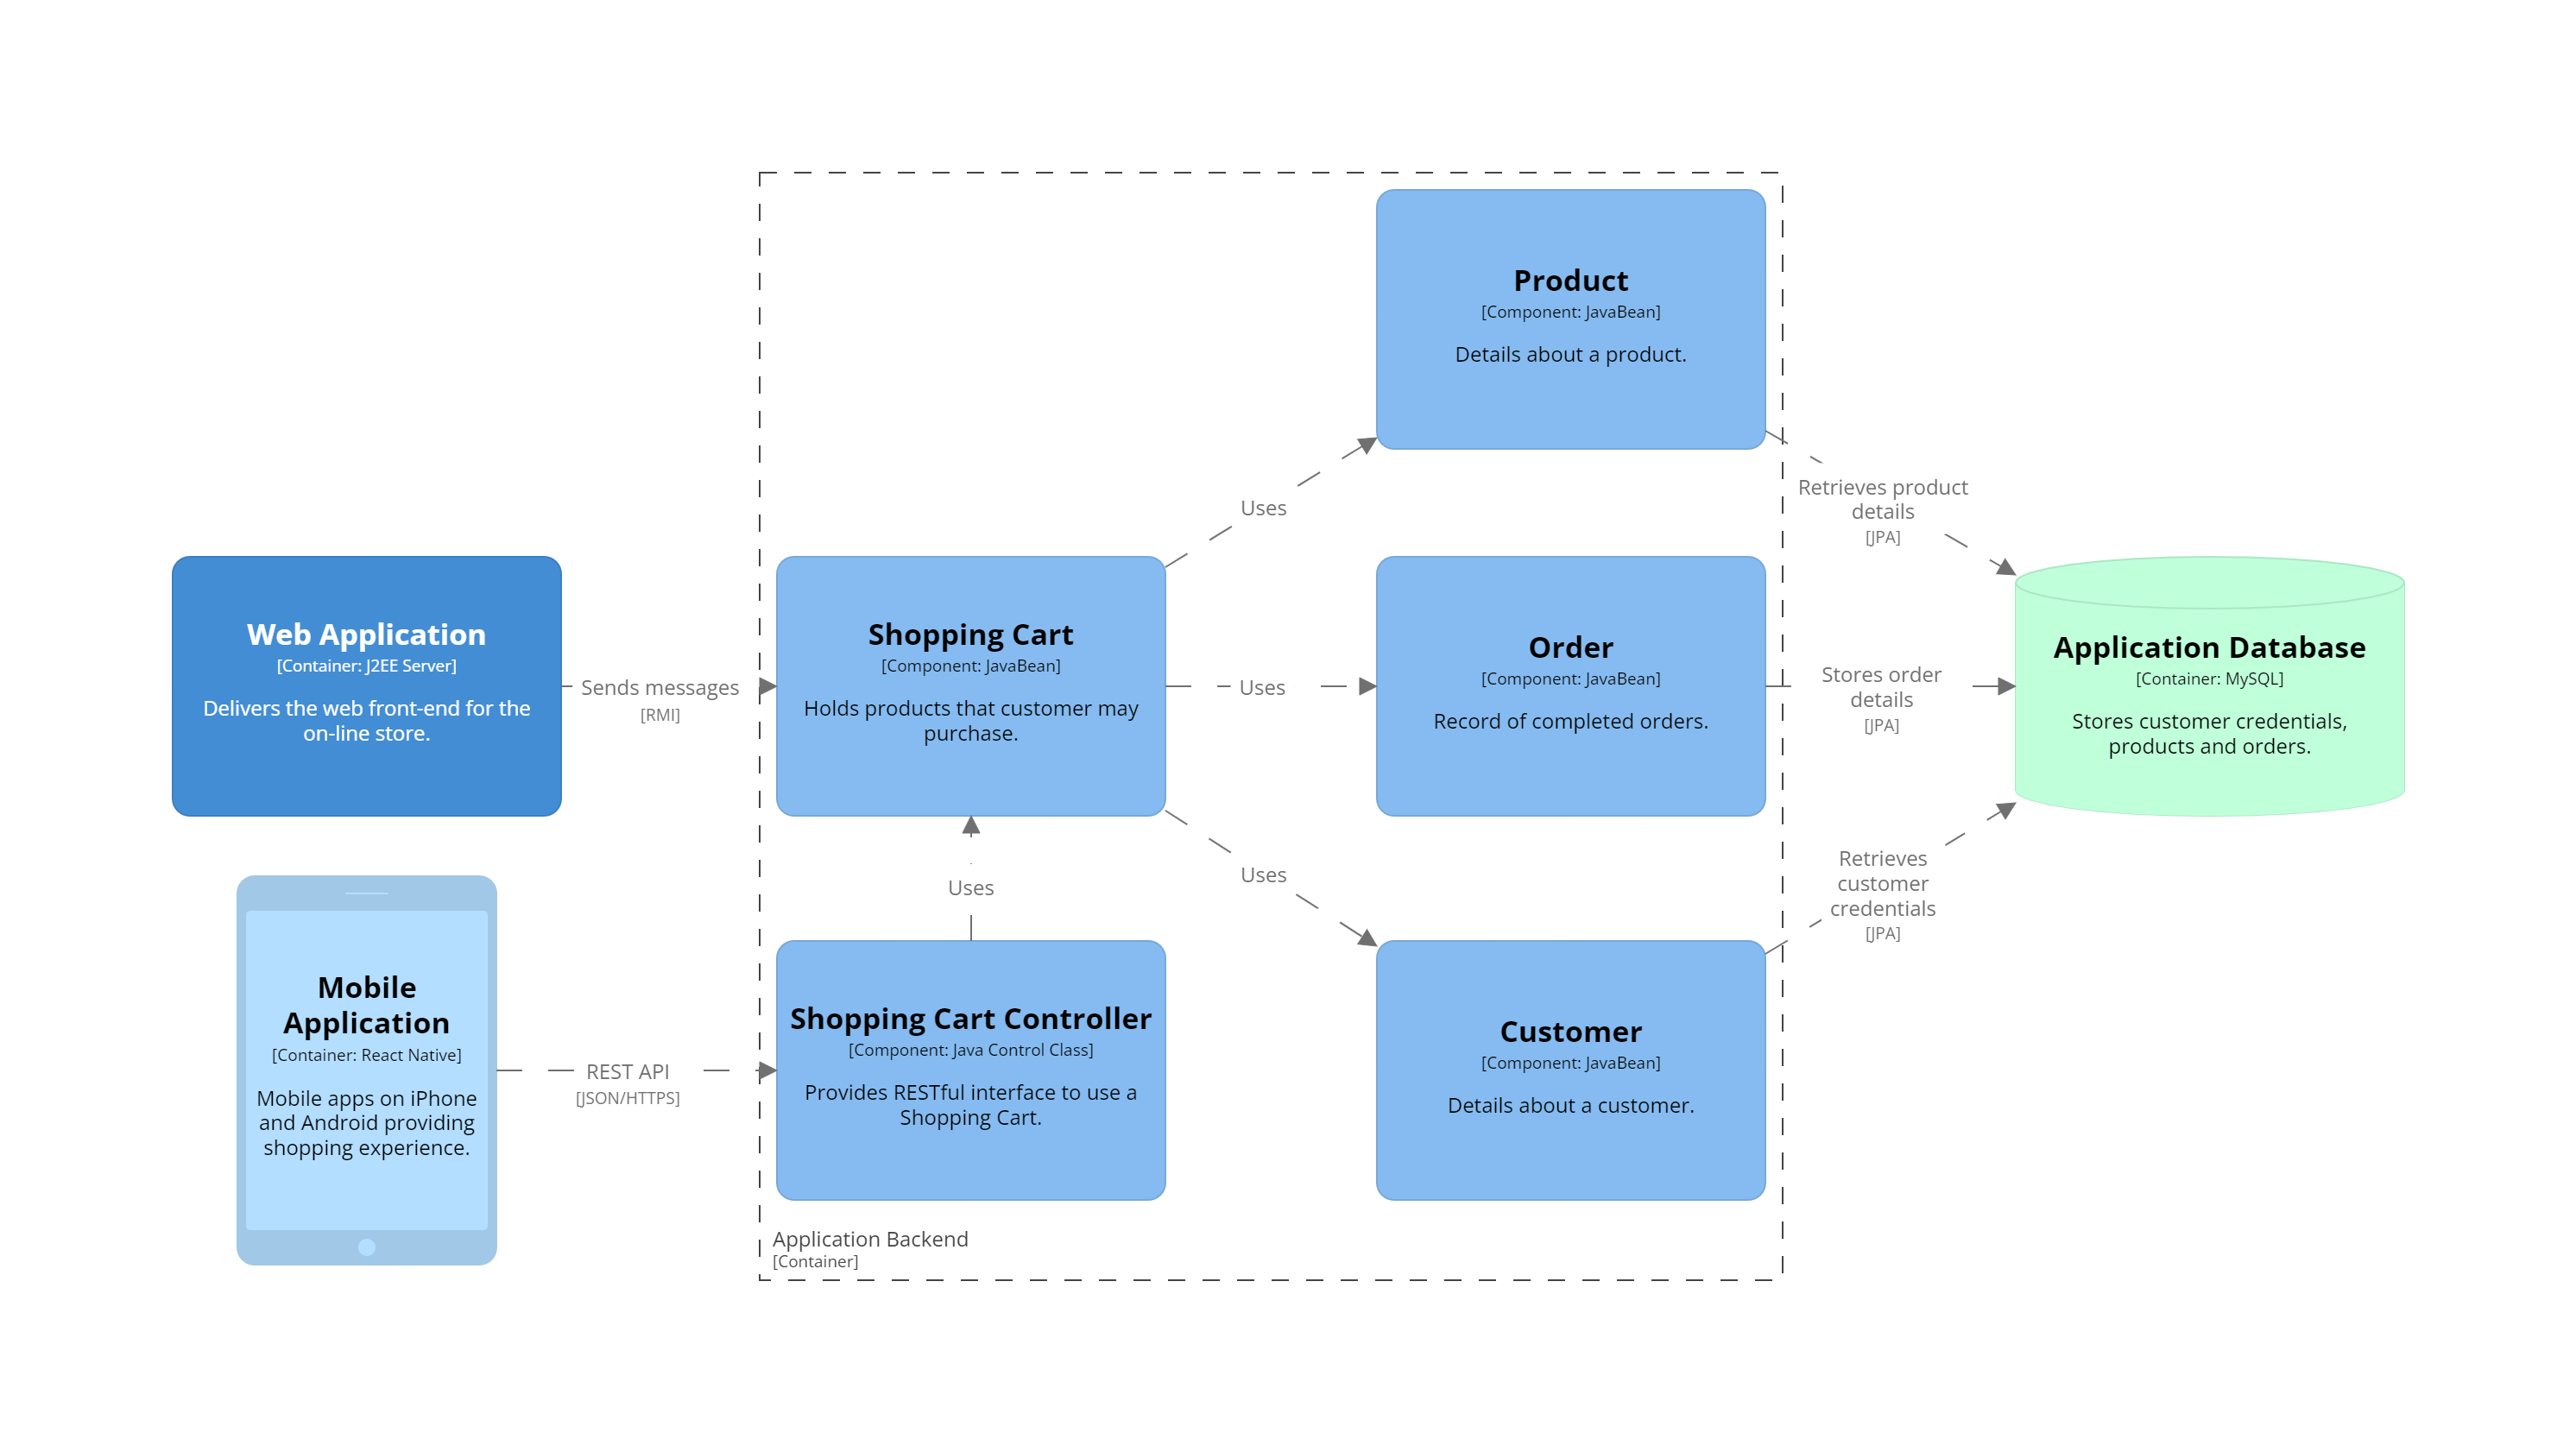
\includegraphics[trim=190 185 197 198,clip,width=0.965\paperwidth]{images/c4/appbackend_component_diagram.png}
    \end{adjustwidth}
    \caption{Component diagram for the application backend container.}
    \label{fig:c4_component_appbackend}
\end{figure}

In figure \ref{fig:c4_component_appbackend}, the application backend is divided into five main components.
The \texttt{Shopping Cart} component provides the backend logic of implementing a shopping cart.
This includes storing the state of the cart in the application database
so that it is available in a later shopping session.
The \texttt{Products} component provides information about products in the application database.
The \texttt{Customers} component retrieves customer credentials from the application database.
The \texttt{Orders} component stores finalised orders in the application database.

\noindent
The web application interacts with the \texttt{Customers}, \texttt{Shopping Cart} and \texttt{Products} components via RMI.
They would provide interfaces for this interaction.
\texttt{Shopping Cart} uses the \texttt{Products}, \texttt{Orders} and \texttt{Customers} components
to deliver its behaviour.
Together they deliver the logical behaviour of providing information about products,
tracking what is in the shopping cart, and placing orders.

The application backend is implemented in Java and uses
\link{JPA Entities}{https://jakarta.ee/specifications/persistence/3.2/jakarta-persistence-spec-3.2.html\#entities}
to manage persistent data in the application database.

The mobile applications use a REST API to communicate with the application backend.
An example of this is shown by the \texttt{Shopping Cart Controller} component
which uses the \texttt{Shopping Cart} to deliver that behaviour to the mobile applications.
Other controllers implementing REST APIs are not shown to reduce the complexity of the diagram.

Figure \ref{fig:c4_component_key}, shows the icons and colours used to represent different elements in the component diagrams. \\

\begin{figure}[h!]
    \centering
    \begin{adjustwidth}{-7.5mm}{-7.5mm}
        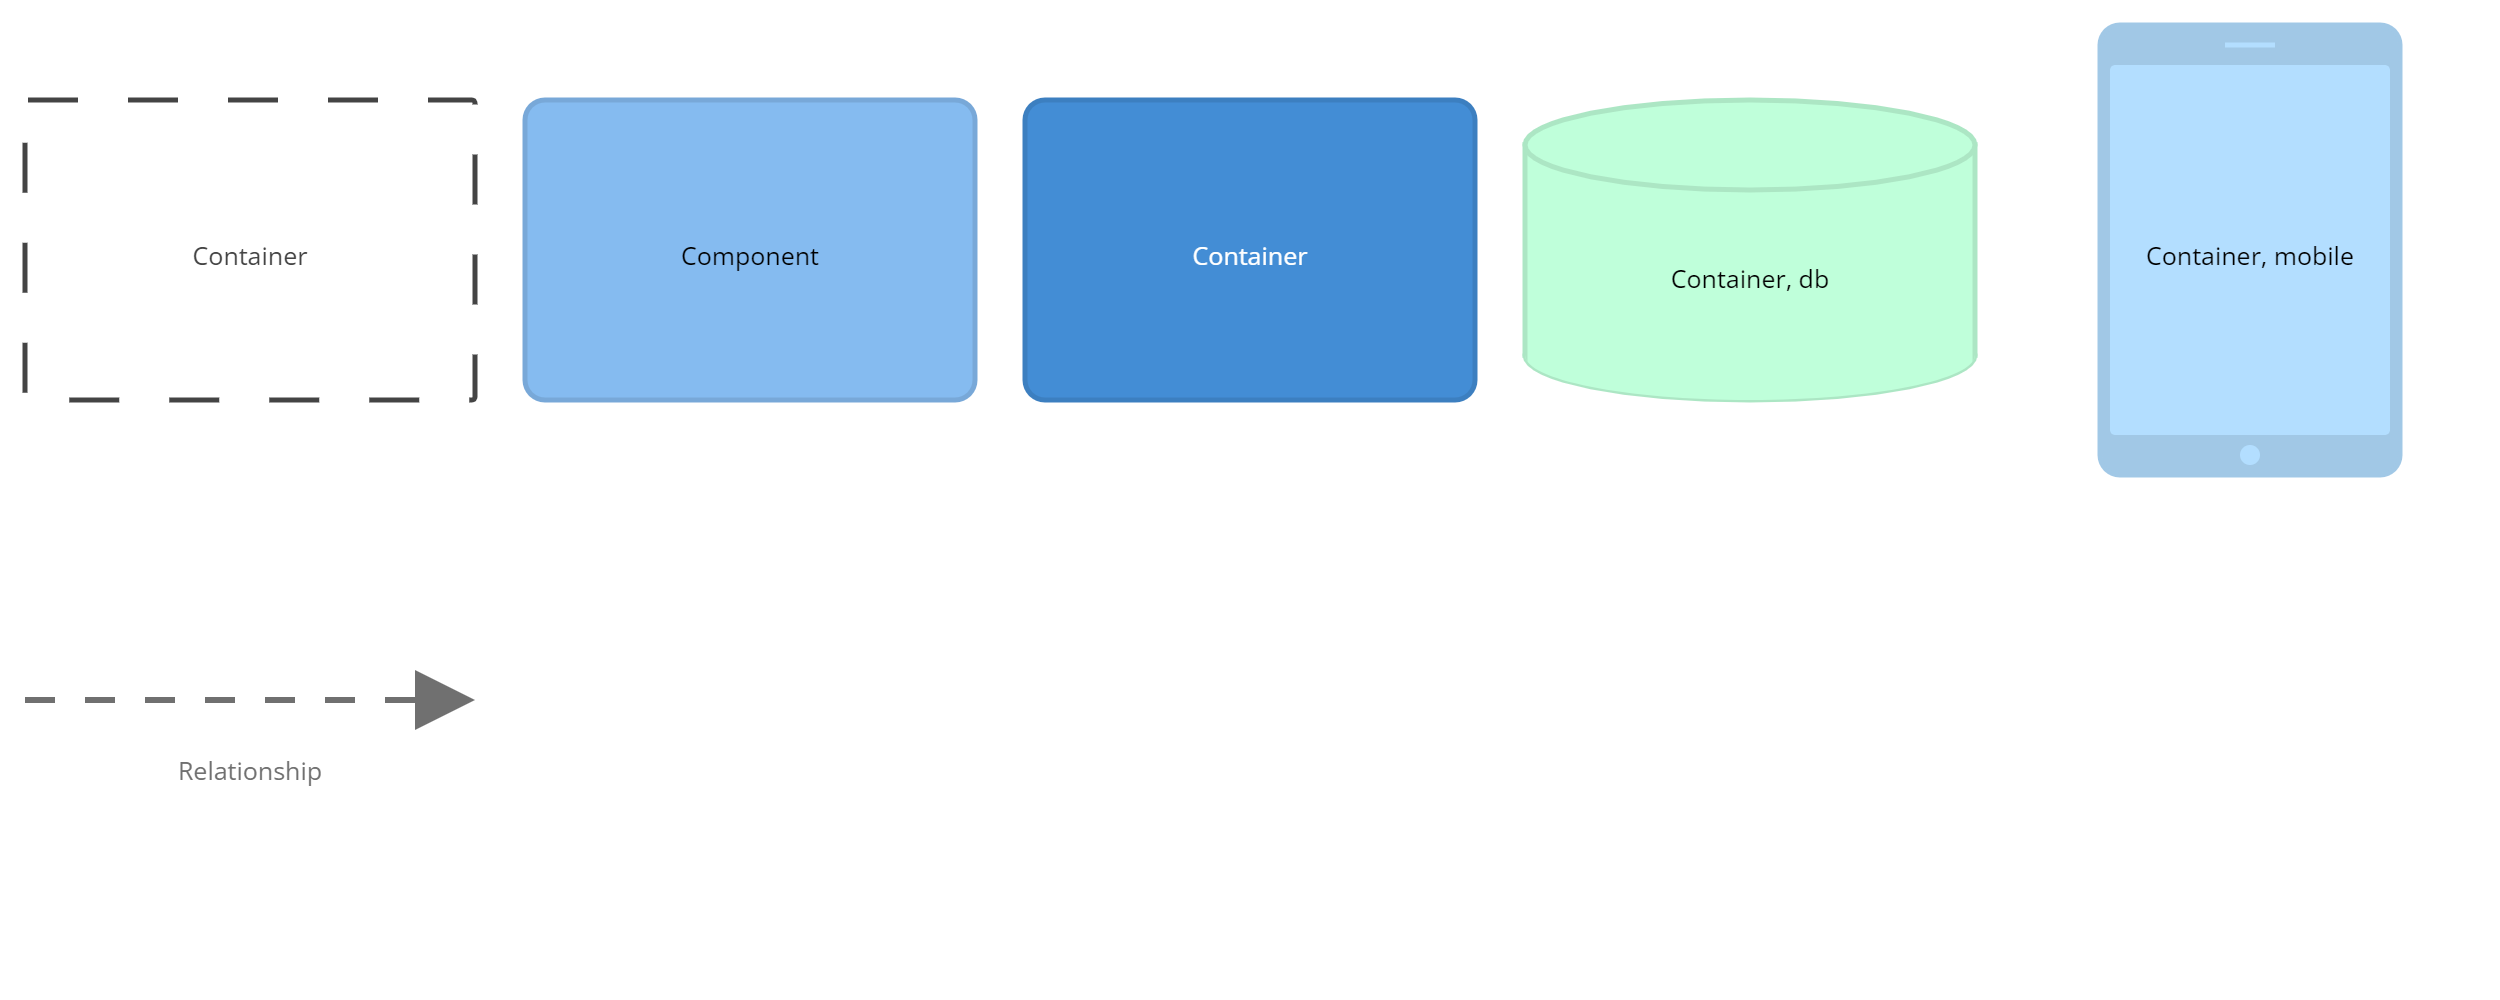
\includegraphics[trim=15 510 90 20,clip,width=0.95\paperwidth]{images/c4/component_diagram-key.png}
    \end{adjustwidth}
    \caption{Component diagram key.}
    \label{fig:c4_component_key}
\end{figure}

\noindent
Figure \ref{fig:c4_component_webapp} shows the components that provide the frontend behaviour,
in the web application,
of browsing for products, adding them to the shopping cart, and purchasing them.

\begin{figure}[h!]
    \centering
    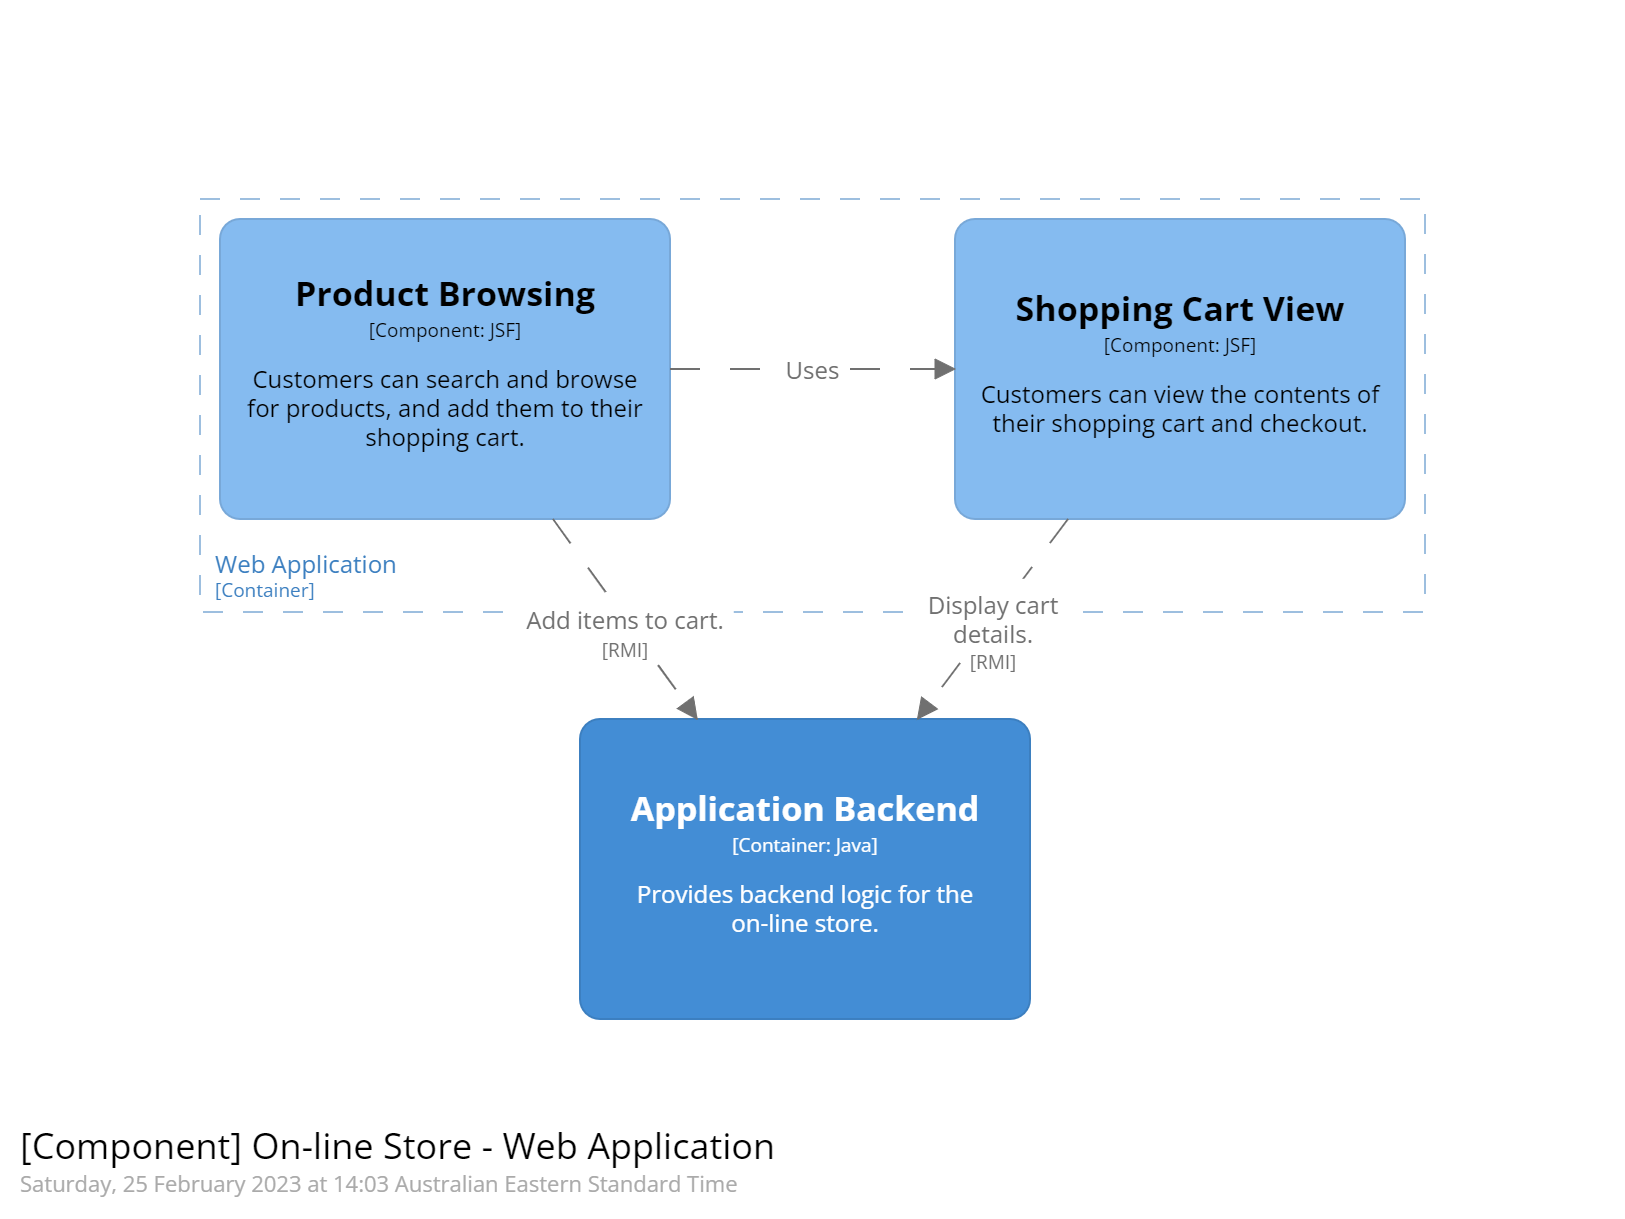
\includegraphics[trim=190 193 190 195,clip,width=0.65\textwidth]{images/c4/webapp_component_diagram.png}
    \caption{Component diagram for the web application container.}
    \label{fig:c4_component_webapp}
\end{figure}

\noindent
Figure \ref{fig:c4_component_browser}, shows that the \texttt{Product Animator} component
is downloaded from the web application to the customer's browser and that it is implemented in JavaScript.
This component provides the code that allows customers to interact with 3D views of products.

\begin{figure}[h!]
    \centering
    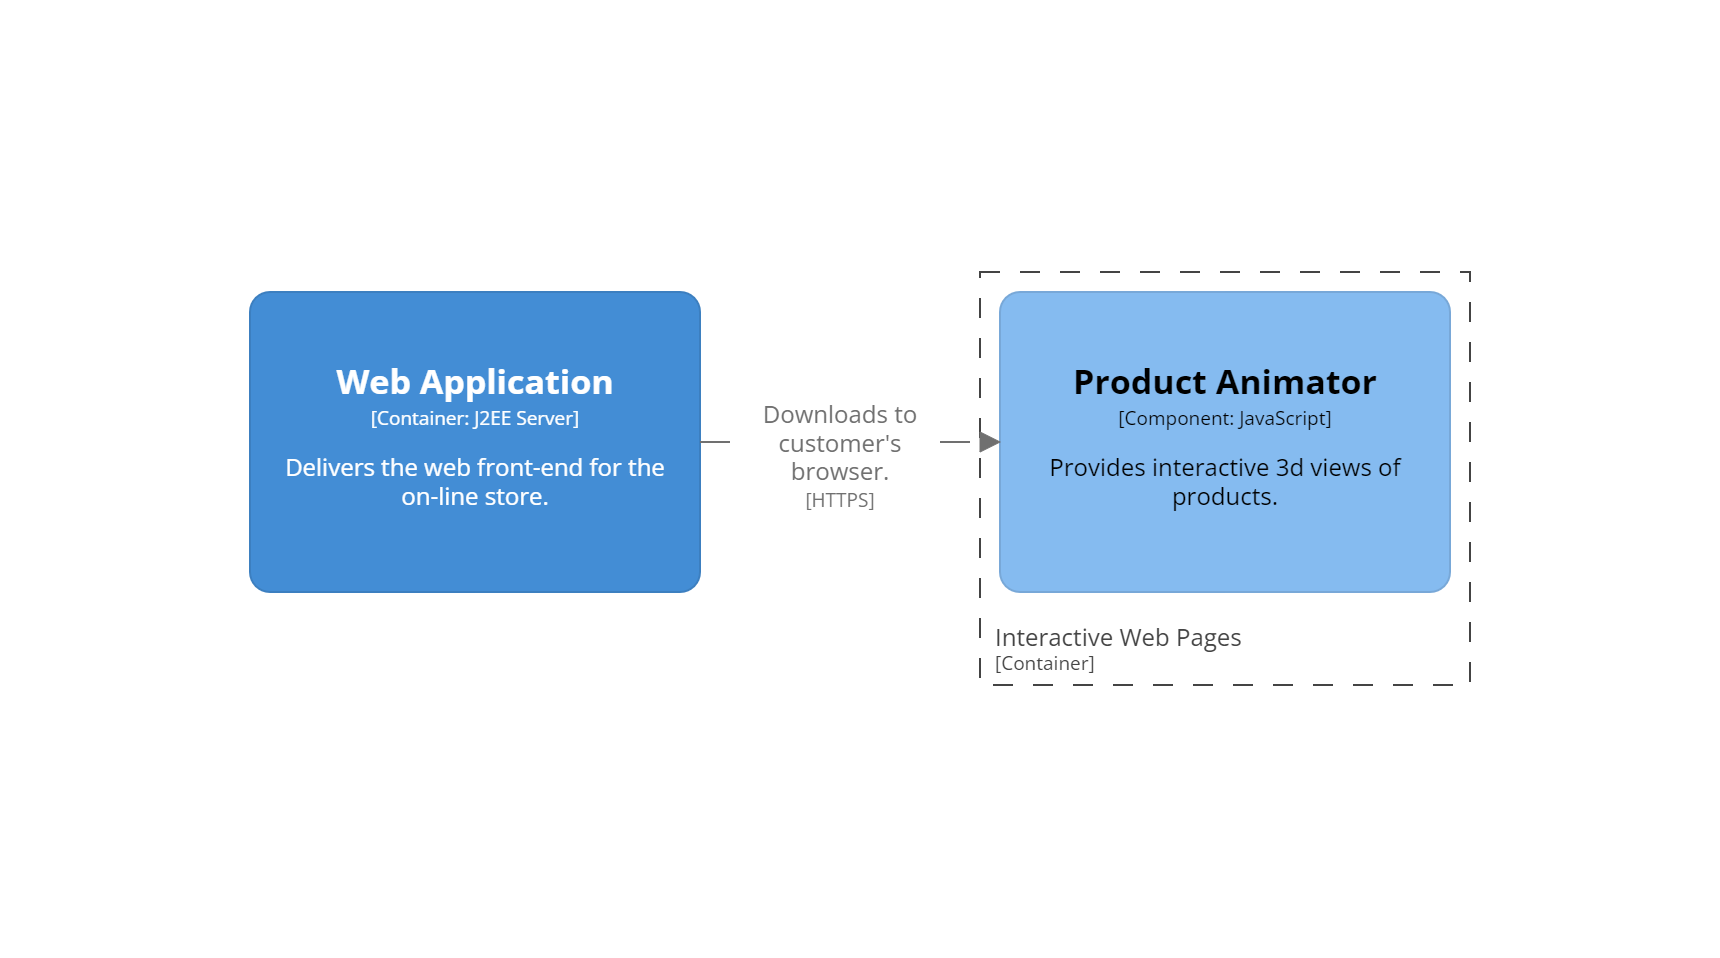
\includegraphics[trim=200 190 195 190,clip,width=0.65\textwidth]{images/c4/browser_component_diagram.png}
    \caption{Component diagram for the interactive web pages container.}
    \label{fig:c4_component_browser}
\end{figure}

\noindent
To keep the example manageable, only the components related to implementing the shopping cart are shown at this level of detail.

\subsubsection{Component Diagram Detail}
There may be some components that are important parts of the software design,
but which may not necessarily be included in component diagrams.
For example, a logging component is an important part of many software systems.
But, due to the nature of a logging component, most other components will use it.
Adding it to component diagrams will usually clutter the diagrams without adding much useful information.
Usually it is better to add a note indicating which logging component is used in the system.
If it is helpful to indicate which components use the logging component,
it may be better to colour code these components or use an icon to represent that they use the logging component.

\subsection{Code}
Code-level diagrams describe the structure of the code that implements a component.
The intent is to provide a visual representation of the important aspects of the code's structure.

C4 does not provide a code level diagram.
It suggests using diagrams appropriate to your programming paradigm.
Assuming the implementation is in an object-oriented language, a
\href{https://www.uml.org/}{UML diagrams}\footnote{Unified Modeling Language [\url{https://www.uml.org/}]}
class diagram would be an appropriate way to model the design of the code.

Figure \ref{fig:classDiagram} is a UML class diagram visualising the static structure
of the classes that implement the \texttt{Shopping Cart} component.
Usually only architecturally significant operations and attributes are shown.
(e.g. Operations and attributes needed to understand relationships and behaviour.)
Rarely do you need to provide all the detail that replicates the source code.
(The source code could be considered a fifth level to the C4 model.)
And for simplicity in this diagram, only the classes and interfaces related to adding items to a shopping cart and checking out are shown.

\begin{figure}[h]
    \centering
    \begin{adjustwidth}{-10.5mm}{-11mm}
        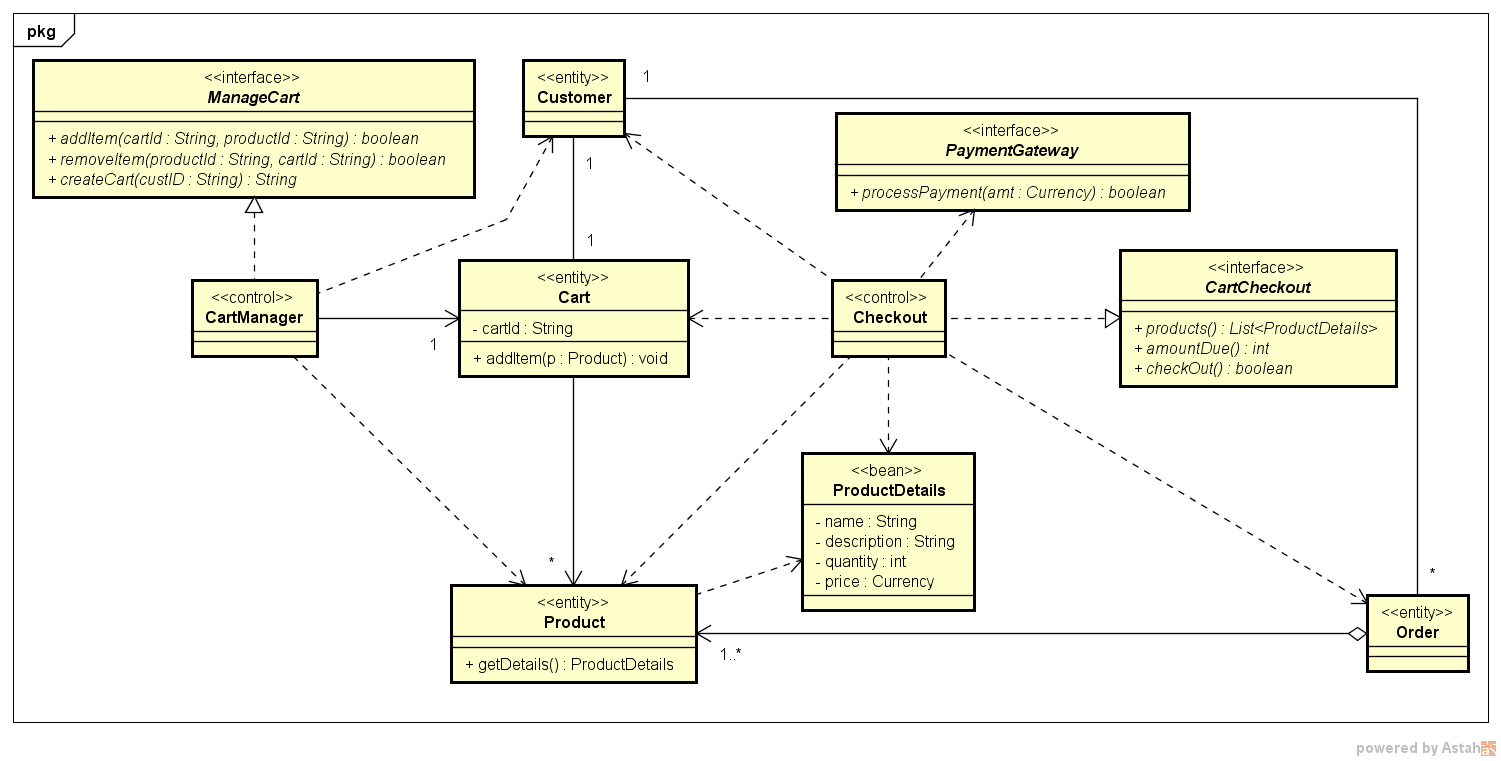
\includegraphics[trim=22 43 22 44,clip,width=0.98\paperwidth]{images/uml/shopping_cart_class_diagram.png}
    \end{adjustwidth}
    \caption{Example static structure for part of the shopping cart component.}
    \label{fig:classDiagram}
\end{figure}

\noindent
The \texttt{CartManager} and \texttt{Checkout} control classes implement, respectively,
the \texttt{\textsl{ManageCart}} and \texttt{\textsl{Cart\-Check\-out}} interfaces.
These two classes implement the Façade design pattern and manage how
adding products to a shopping cart and checking out are delivered by the classes in this package.
Going back to the application backend and web application component diagrams
(figures \ref{fig:c4_component_appbackend} and \ref{fig:c4_component_webapp}),
when a customer, via their web browser, selects to add a product to their shopping cart,
the \texttt{Product Browsing} component's logic uses the \texttt{\textsl{ManageCart}}
interface's \texttt{\textsl{additem}} operation to send a message to the \texttt{Shopping Cart} component.

In the implementation of the \texttt{Shopping Cart} component,
the \texttt{CartManager} class uses the \texttt{EntityManager}
to load the product details and the customer's shopping cart from the application database.
The \texttt{EntityManager} creates the \texttt{Product} and \texttt{Cart} entity objects,
and \texttt{CartManager} adds the product to the cart.
Once this is done the \texttt{EntityManager} is used to save the updated cart data into the database.

When a customer wants to checkout the products in their shopping cart, the \texttt{Shopping Cart View} component
uses the \texttt{\textsl{CartCheckout}} interface's \texttt{\textsl{products}} operation
to get a list of the product details to be displayed in the shopping cart.
The \texttt{ProductDetails} class is a Java bean that is used to pass the data about each product to the \texttt{Shopping Cart View}.
Once a customer decides to buy the products in their shopping cart,
the \texttt{Shopping Cart View} sends the \texttt{checkOut} message to the \texttt{Shopping Cart}.
\texttt{Checkout} uses the \texttt{\textsl{PaymentGateway}} interface to process the payment.

\subsubsection{Class Diagram Notation}\label{sec:classNotation}
Formally in UML, rectangles represent \emph{classifiers}. A \emph{class} is one type of classifier.
In a class diagram, a rectangle represents a class, unless a keyword is used to indicate that it is a different type of classifier.
Classifier rectangles have three compartments.
The top compartment contains its name and optionally includes a keyword, stereotypes and properties for the classifier.
The middle compartment contains \emph{attributes}.
The bottom compartment contains \emph{operations}.

Solid lines represent \emph{associations}, which may optionally have an arrow indicating the direction of the relationship.
An association indicates a structural relationship between classes.
Typically this means that the target of an association will be an implicit attribute of the class.
The end of an association can use \emph{multiplicity} to indicate the number of objects of the class that may take part in the relationship.

A diamond on the end of an association indicates an \emph{aggregate} relationship.
The diamond is on the end that is the aggregate, and the other end is the part.
The diamond may be filled or not. A filled diamond represents \emph{composition}.
This indicates `ownership', where the aggregate controls the lifespan of the part.
A hollow diamond, as in the relationship between \texttt{Order} and \texttt{Product},
indicates \emph{aggregation}.
This is a weaker relationship than composition, as the aggregate does not control the lifespan of the part,
but it still indicates a strong relationship between the classes.

A dashed line with an open arrowhead (e.g. from \texttt{CartManager} to \texttt{Product})
indicates that one classifier \emph{depends} on (or uses) another. This is meant to indicate a transient relationship.

A dashed lines with a closed and hollow arrowhead (e.g. from \texttt{Checkout} to \texttt{\textsl{CartCheckout}})
indicates that the class is \emph{realising} (or implementing) that interface.

\textit{Italicised} names indicate an abstract classifier. Keywords are used to indicate the type of a classifier.
In this example, the keyword \guillemotleft interface\guillemotright~indicates that the classifier is an interface.
Stereotypes use the same notation as keywords. Three standard stereotypes for classes in UML are:
\begin{description}[nosep,left=5mm]
    \item[\guillemotleft entity\guillemotright] Represents a concept (\emph{entity}) from the problem domain.
    \item[\guillemotleft control\guillemotright] Provides logical behaviour from the solution domain.
    \item[\guillemotleft boundary\guillemotright] Communicates with something outside of the system. (Not shown in diagram.)
\end{description}
An additional stereotype \guillemotleft bean\guillemotright~is used to indicate that the class is a Java bean.

\subsection{Dynamic}
Dynamic diagrams in C4 show how different parts of the model collaborate to deliver architecturally significant requirements.
Normally dynamic diagrams are used to describe behaviour that is not clear from other diagrams and descriptions.
This can include complex interactions between modules, complex concurrency, real-time constraints, or latency constraints.

For example, when Boeing was upgrading the combat control system of the
\link{F-111}{https://www.youtube.com/watch?v=xUcpZJE050s}
for the Australian Airforce, they designed a software architecture that used
\href{https://www.ibm.com/docs/en/integration-bus/9.0.0?topic=corba-common-object-request-broker-architecture}{CORBA}%
\footnote{Common Object Request Broker Architecture [\url{https://www.ibm.com/docs/en/integration-bus/9.0.0?topic=corba-common-object-request-broker-architecture}]}
as middleware.
The implementation of the middleware caused a fixed delay in sending messages between components.
From an architectural design perspective,
it was important to document this delay and enforce a maximum delay on the time taken to complete any process.
This type of constraint can be documented with a dynamic diagram and supporting documentation.

Figure \ref{fig:c4_dynamic} provides an overview of how the
\texttt{Product Browsing} component in the \texttt{Web Application} container collaborates with the
\texttt{Shopping Cart} component in the \texttt{Application Backend} container
to deliver the behaviour of a customer adding a product to their shopping cart.
It also shows the communication between the \texttt{Shopping Cart} component and the application database.

\begin{figure}[h!]
    \centering
    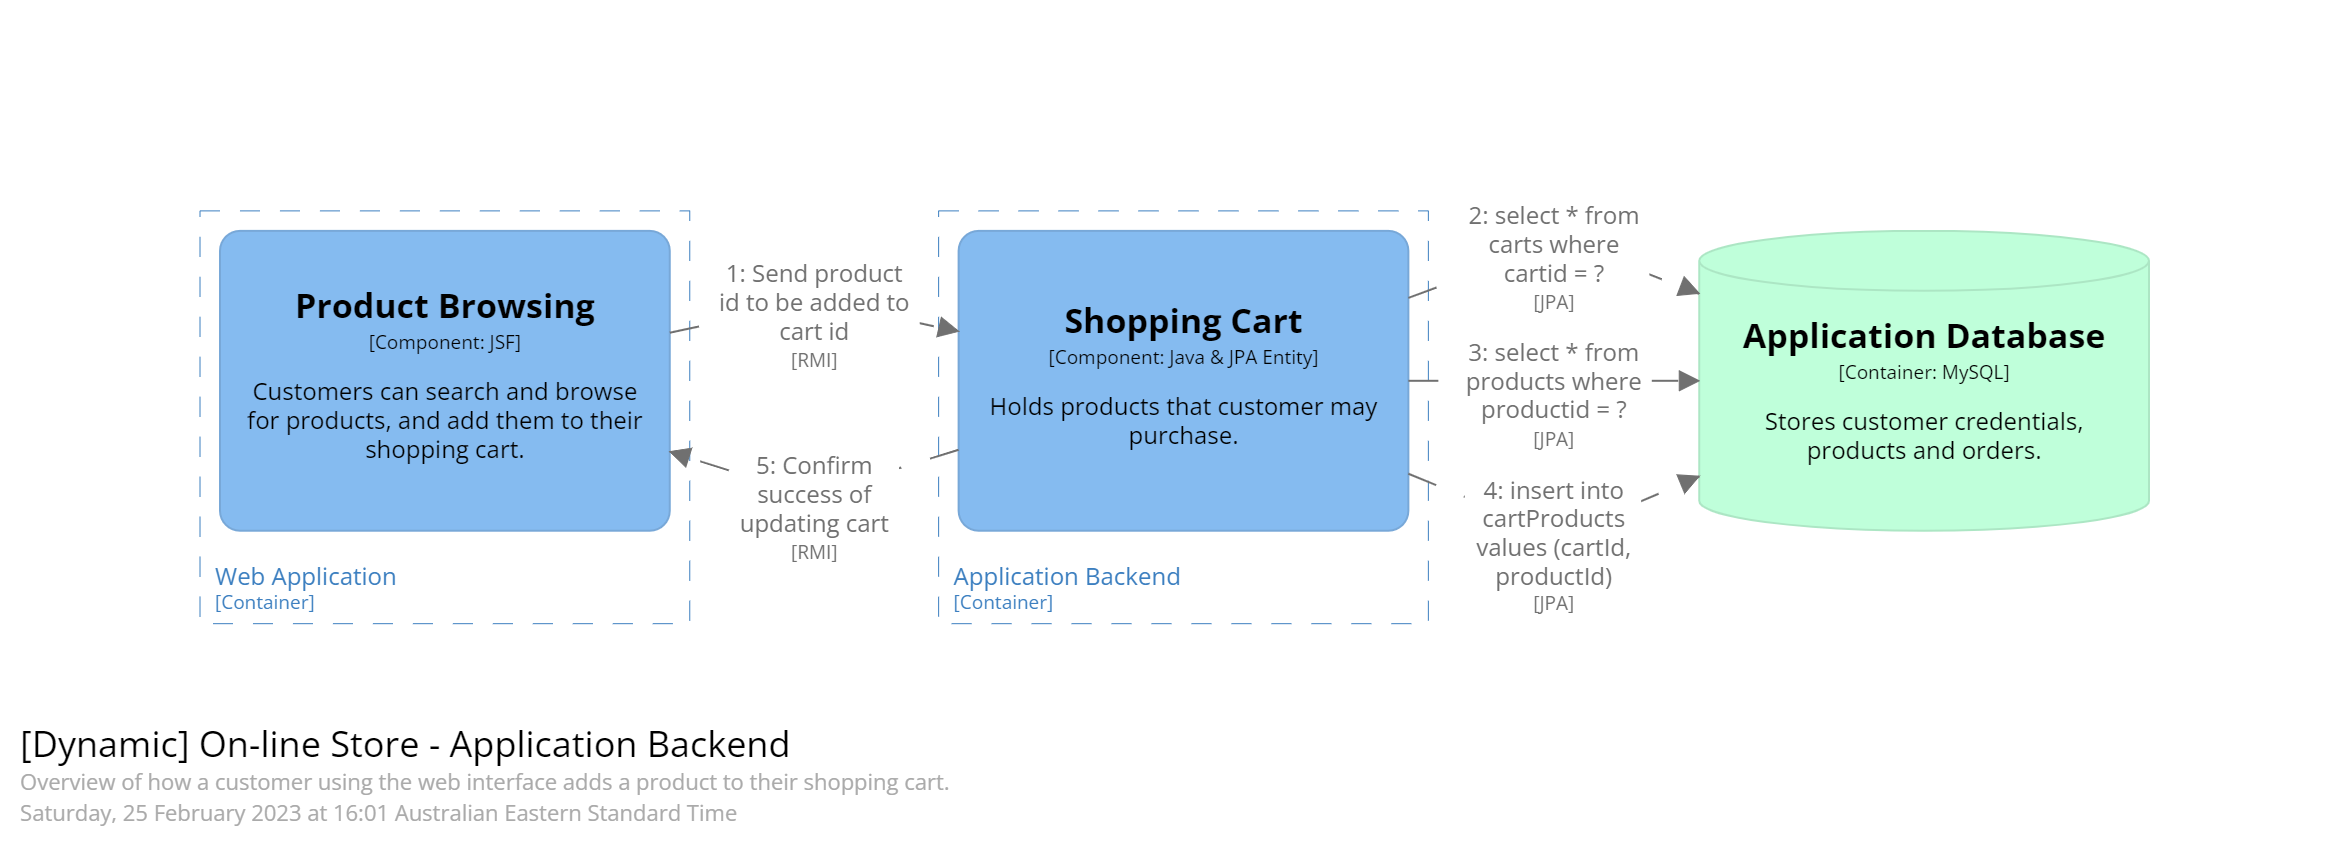
\includegraphics[trim=175 220 197 185,clip,width=\textwidth]{images/c4/add_to_cart_dynamic_diagram.png}
    \caption{Dynamic diagram for adding a product to the customer's shopping cart.}
    \label{fig:c4_dynamic}
\end{figure}

\noindent
A dynamic diagram should provide enough information to clarify any requirements or constraints on the design,
but should not be so restrictive as to limit valid implementation choices.

UML provides two types of interaction diagrams that are similar to dynamic diagrams.
A communication diagram is very similar to a dynamic diagram.
A sequence diagram focusses on the time or ordered sequence of events that occur in a scenario.
In documenting a software architecture,
there may be some types of constraints that are more clearly expressed through a sequence diagram.

\subsubsection{Detailed Behaviour}\label{sec:detailedSeqDiagram}
\begin{figure}[h!]
    \centering
    \begin{adjustwidth}{-11mm}{-11mm}
        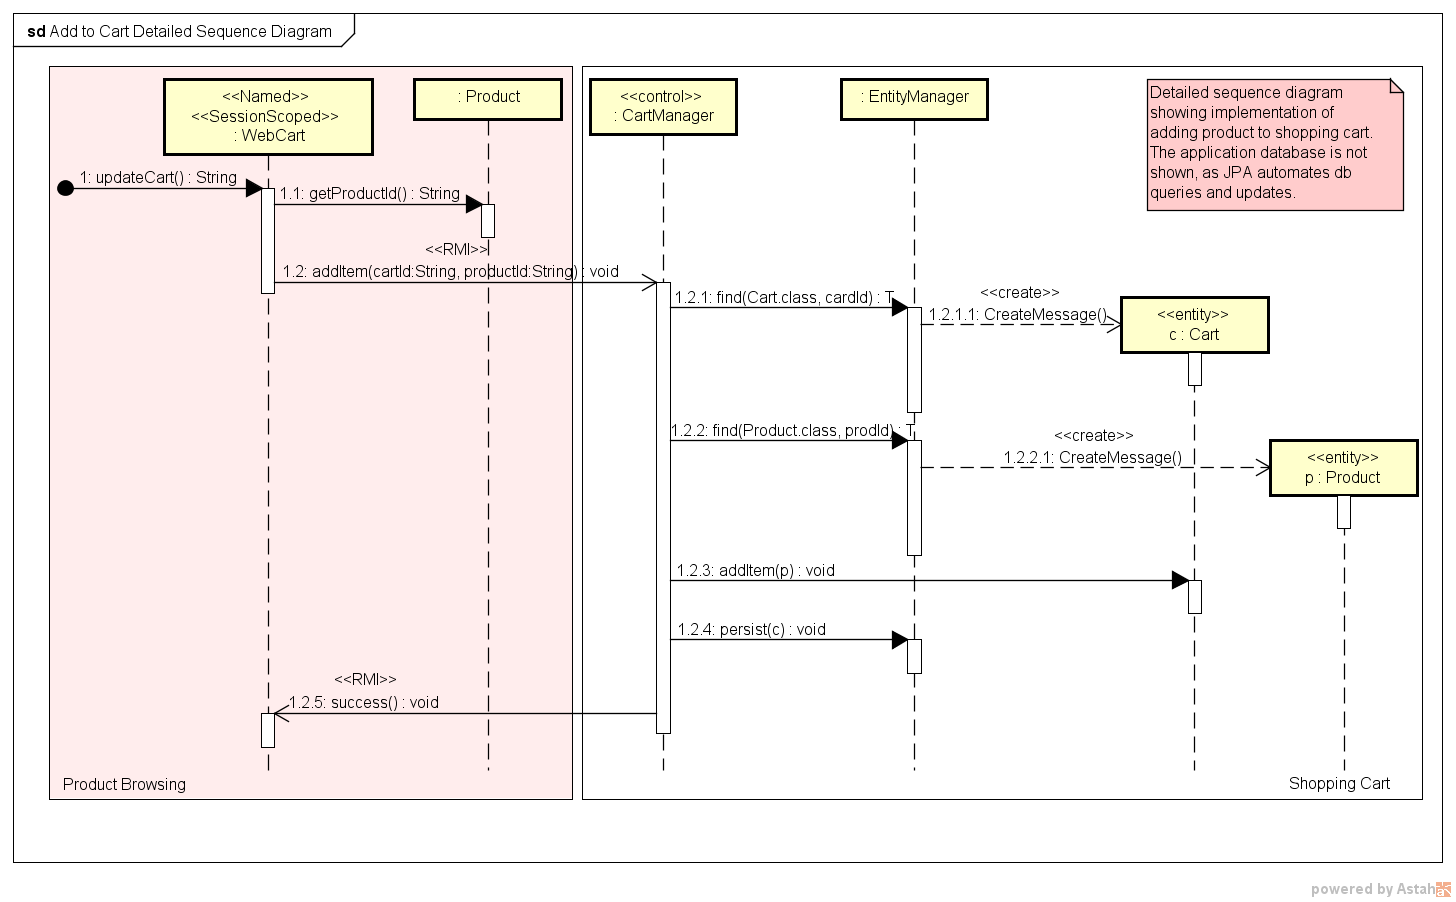
\includegraphics[trim=35 69 24 47,clip,width=0.98\paperwidth]{images/uml/detailed_sequence_diagram.png}
    \end{adjustwidth}
    \caption{Example detailed sequence diagram showing the implementation of customer adding a product to their shopping cart.}
    \label{fig:detailedSequenceDiagram}
\end{figure}

\noindent
Figure \ref{fig:detailedSequenceDiagram} is a detailed sequence showing how the class model in
figure \ref{fig:classDiagram} implements the behaviour of a customer adding a product to their shopping cart.
This is a more detailed, or code-level, view of the scenario of adding a product to a customer's shopping cart shown in figure \ref{fig:c4_dynamic}.
You would only provide detailed behavioural diagrams to describe architecturally important details of the detailed design.

The scenario starts with the JSF session-scoped bean \texttt{WebCart} receiving the \texttt{updateCart} message from the browser.
\texttt{WebCart} retrieves the product id and uses the \texttt{ManageCart} interface to send it, along with the cart id,
to the \texttt{Shopping Cart} component in the application backend.
The \texttt{\textsl{ManageCart}} interface is implemented by the \texttt{CartManager} class in the \texttt{Shopping Cart} component.

The \texttt{CartManager} uses the JPA \texttt{EntityManager} to retrieve the cart and product entities from the application database.
Once the product is added to the cart, the \texttt{EntityManager} saves the updated cart details to the database.
Upon successfully saving the updated cart, the \texttt{CartManager} notifies the \texttt{WebCart} object
in the \texttt{Product Browsing} component in the web application.

\subsubsection{Sequence Diagram Notation}
Sequence diagrams are read from the top down.
The top of the diagram represents the start of the scenario, and execution time progresses down the diagram.
The bottom of the diagram is the end of the scenario.
Duration constraints can be placed between messages indicating information like the maximum allowed time between the start and end of a message.

Rectangles with dashed lines descending from them are \emph{lifelines}.
They represent an instance of a participant in the scenario being described.
The name at the top of a lifeline describes the participant.
In figure~\ref{fig:detailedSequenceDiagram}, these are objects of classes from the detailed design.
The class diagram in figure~\ref{fig:classDiagram} shows the classes for the detailed design of the \texttt{Shopping Cart} component used in this scenario.

The horizontal lines are \emph{messages} sent between participants.
Messages use hierarchical numbers to indicate both nesting and sequence of messages.
Message 1.1 is sent by message 1. Message 1.1.1 comes before message 1.1.2.
Message 1 in figure~\ref{fig:detailedSequenceDiagram} is a \emph{found message},
meaning that the sender of the message is not shown in the diagram.

A closed arrowhead on a message (e.g. message 1.1) indicates that it is a synchronous message.
An open arrowhead on a message (e.g. message 1.2) indicates that it is an asynchronous message.
In figure~\ref{fig:detailedSequenceDiagram}, stereotypes have been placed on messages between containers
(i.e. messages 1.2 and 1.2.5) to indicate the protocol used to send the message.

The vertical rectangles sitting on top of lifelines are \emph{execution specifications}.
They indicate when an instance is executing logic.
For example, after the asynchronous message 1.2 is sent to the \texttt{CartManager} object,
message 1 finishes executing.
When the synchronous message 1.2.1 is sent to the \texttt{EntityManager}, message 1.2 is still active
as it is waiting for message 1.2.1 to finish before message 1.2 can continue to the next part of the logic.

The \guillemotleft create\guillemotright~stereotype indicates when an instance is created.
When an instance is created, its lifeline starts at the level of the sequence diagram that indicates the point in time when it is created.
When an instance is destroyed, its lifeline finishes, with a large \texttt{X}.
Lifelines that are at the top of the diagram indicate instances that existed before the start of the scenario.
Lifelines that reach the bottom of the diagram indicate instances that still exist after the end of the scenario.

System boundary boxes in figure \ref{fig:detailedSequenceDiagram} indicate the components being implemented by the objects.
The \texttt{Product Browsing} component is shaded in pink.
The \texttt{Shopping Cart} component is white.

\subsection{Deployment}\label{sec:c4_deployment}
While not one of the ``four C's'', deployment diagrams are important for most systems.
They describe the physical architecture or infrastructure on which the system will be deployed.
It shows which containers will run on which computing platforms (\emph{deployment nodes}).
Deployment nodes can be nested, as shown in figure \ref{fig:c4_deployment}.
They may also contain infrastructure nodes or software system instances\footnote{\url{https://docs.structurizr.com/dsl/language\#deploymentnode}}.

\begin{figure}[h!]
    \centering
    \begin{adjustwidth}{-7.5mm}{-7.5mm}
        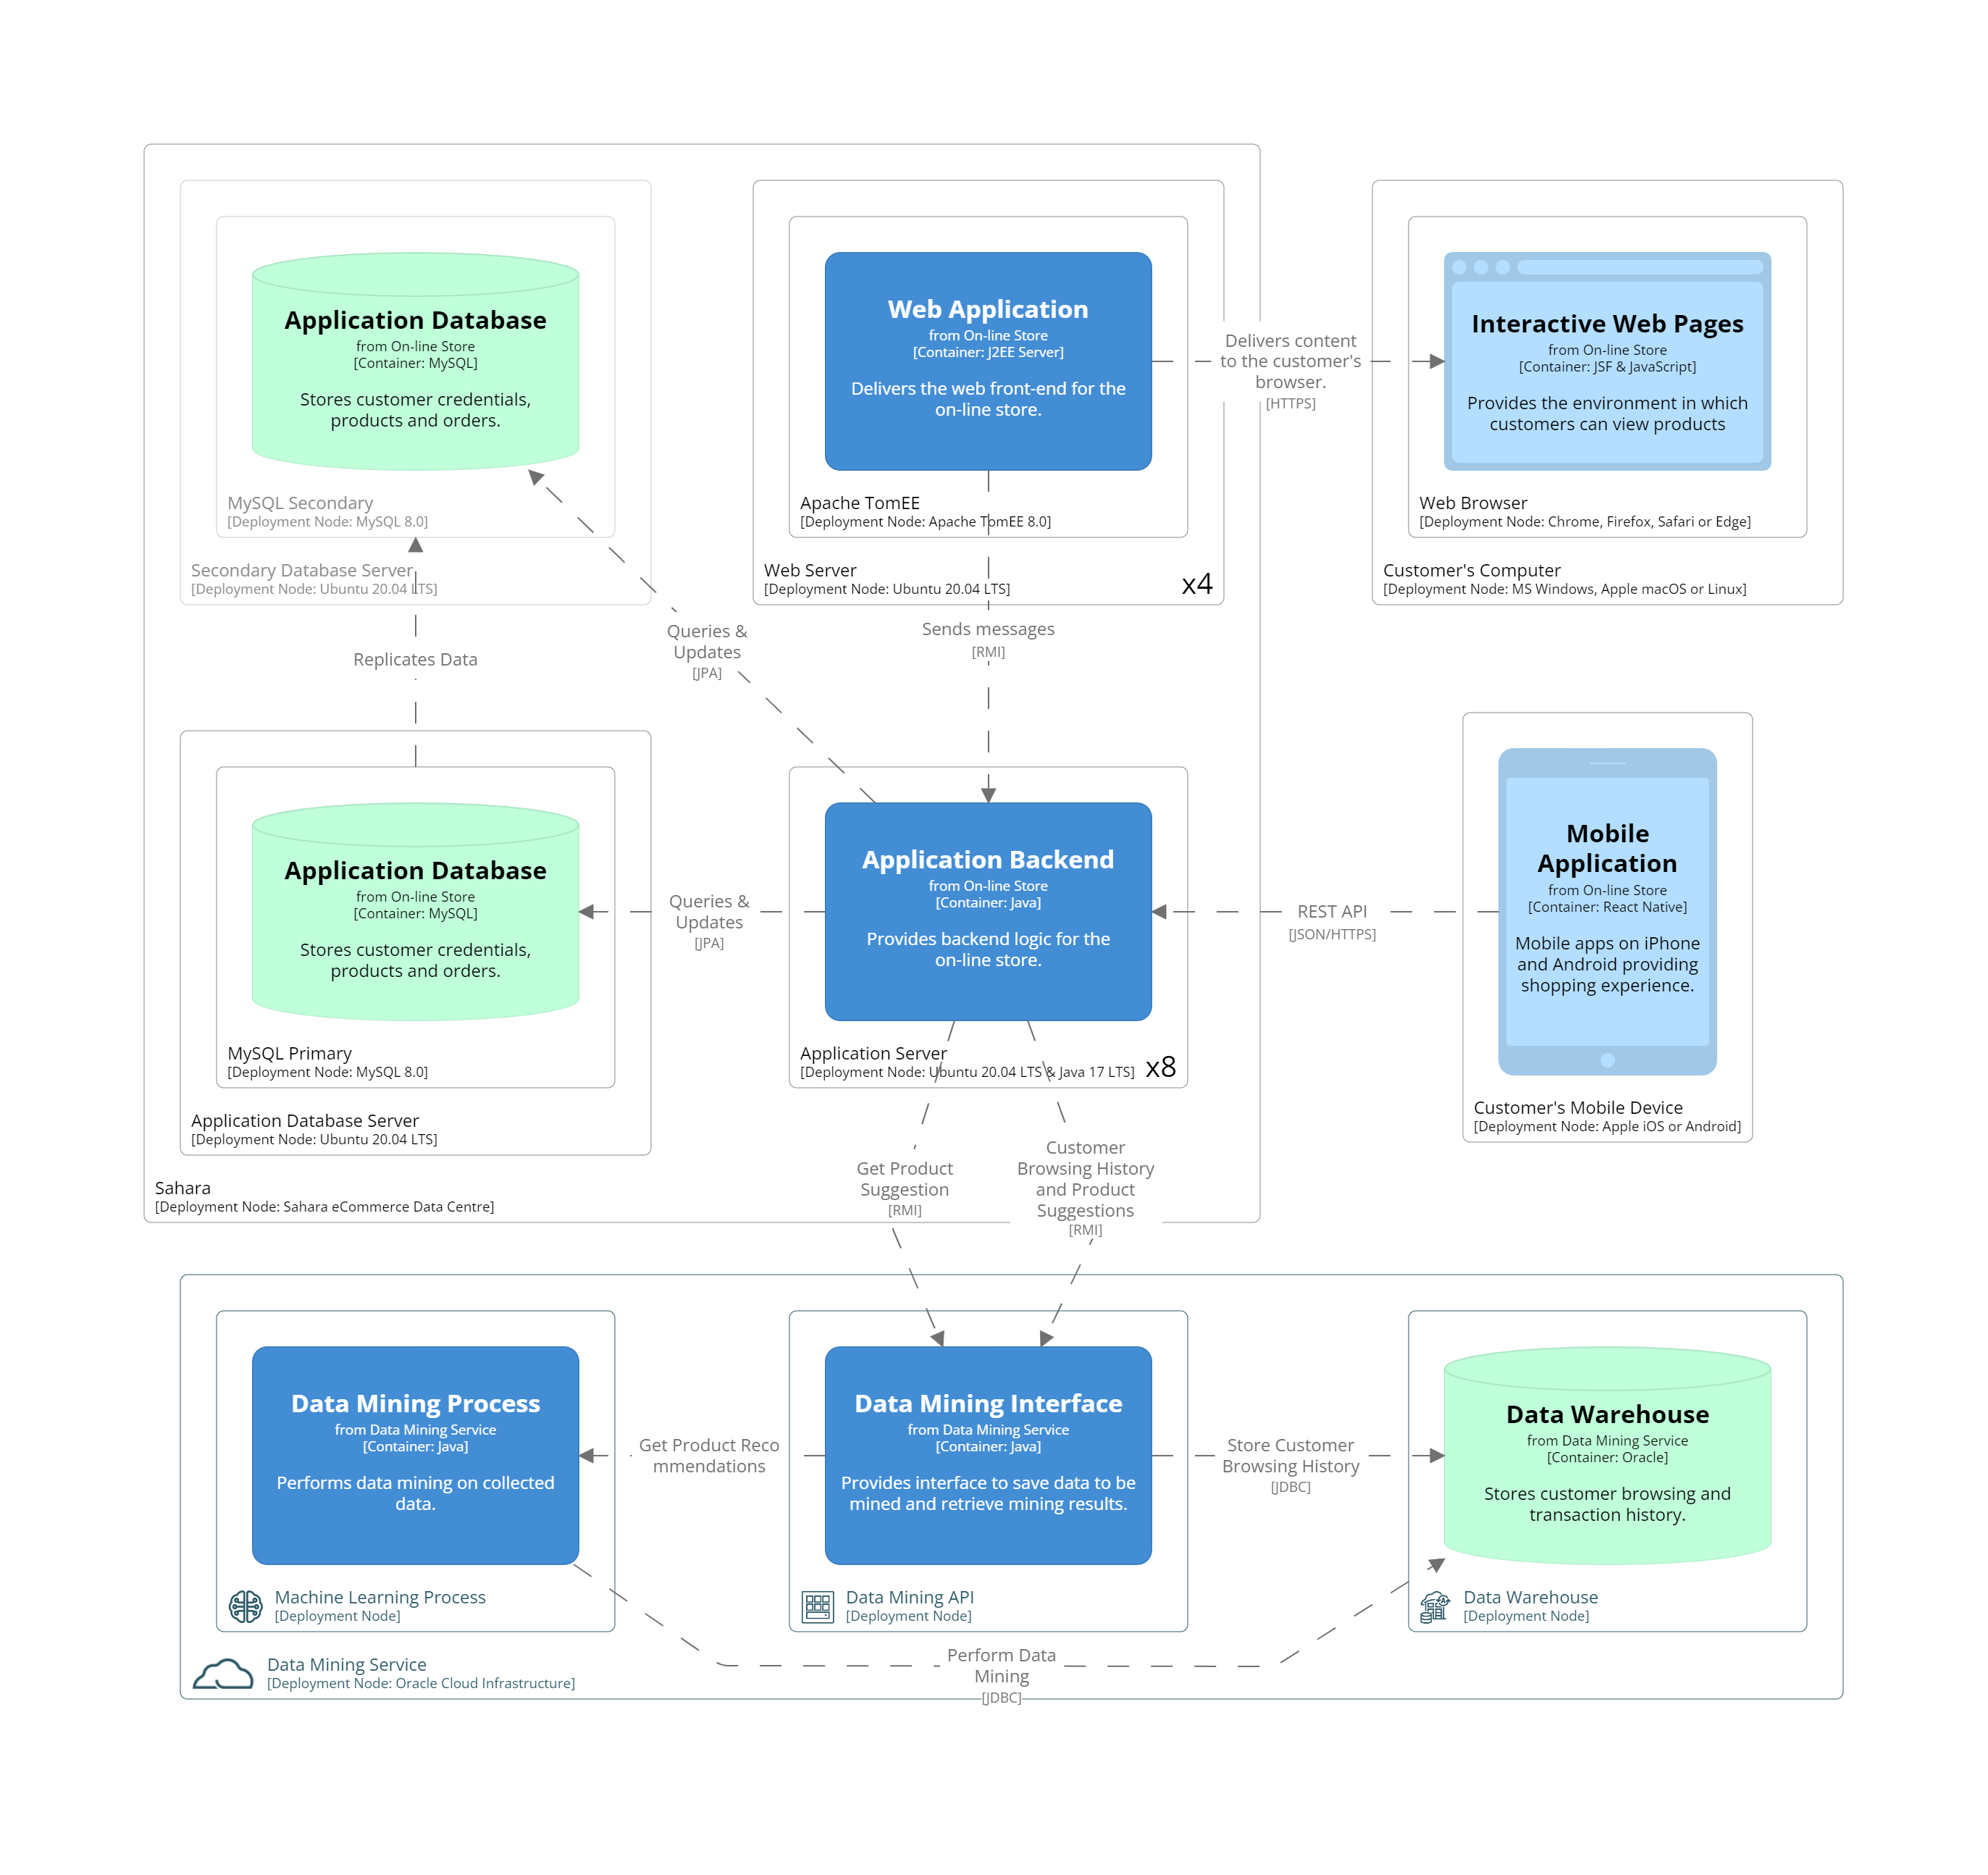
\includegraphics[trim=195 235 195 198,clip,width=0.95\paperwidth]{images/c4/deployment_diagram.png}
    \end{adjustwidth}
    \caption{Deployment diagram for the Sahara eCommerce System.}
    \label{fig:c4_deployment}
\end{figure}

\noindent
Figure \ref{fig:c4_deployment} is an example C4 deployment diagram for the Sahara eCommerce system.
It shows that the on-line store software system runs in Sahara's data centre.
The data mining service runs on Oracle's cloud infrastructure.
This approach of a system that uses cloud services for some of its implementation is called a \emph{hybrid cloud} application.
There are also the apps running on mobile devices and the code running in the customer's browser.

A software environment is embedded in the hardware environment on which it runs.
The web application runs in an \link{Apache TomEE}{https://tomee.apache.org/} J2EE server, which is running on a Ubuntu server.
The ``\texttt{x4}''\footnote{It is an unfortunate constraint of C4 that this must be an explicit number.
That is fine for a system hosted on an organisation's own infrastructure, as they need to know how many servers need to be provisioned.
If you are running virtual servers, this is less informative and does not clearly show capability of spinning up
servers as needed, or spinning them down when not needed.}
inside the web server deployment node indicates that there will be four of these servers to share the load.
The application backend runs on eight Ubuntu servers, providing the core business logic shared by the web and mobile applications.

The application database runs in MySQL on its own Ubuntu server.
The application database is replicated on another server, allowing for failover.
The application backend can continue to operate if the primary application database fails.

The application backend communicates with the data mining service
through an API published by the data mining interface running in a virtual machine on Oracle's cloud infrastructure.
The data mining service uses Oracle's machine learning services to perform the data mining.
Oracle's cloud-based data warehouse infrastructure is used to hold all the data.

Figure \ref{fig:c4_deployment_key} is the key describing the icons and colours used in the deployment diagram.

\begin{figure}[h!]
    \centering
    \begin{adjustwidth}{-7.5mm}{-7.5mm}
        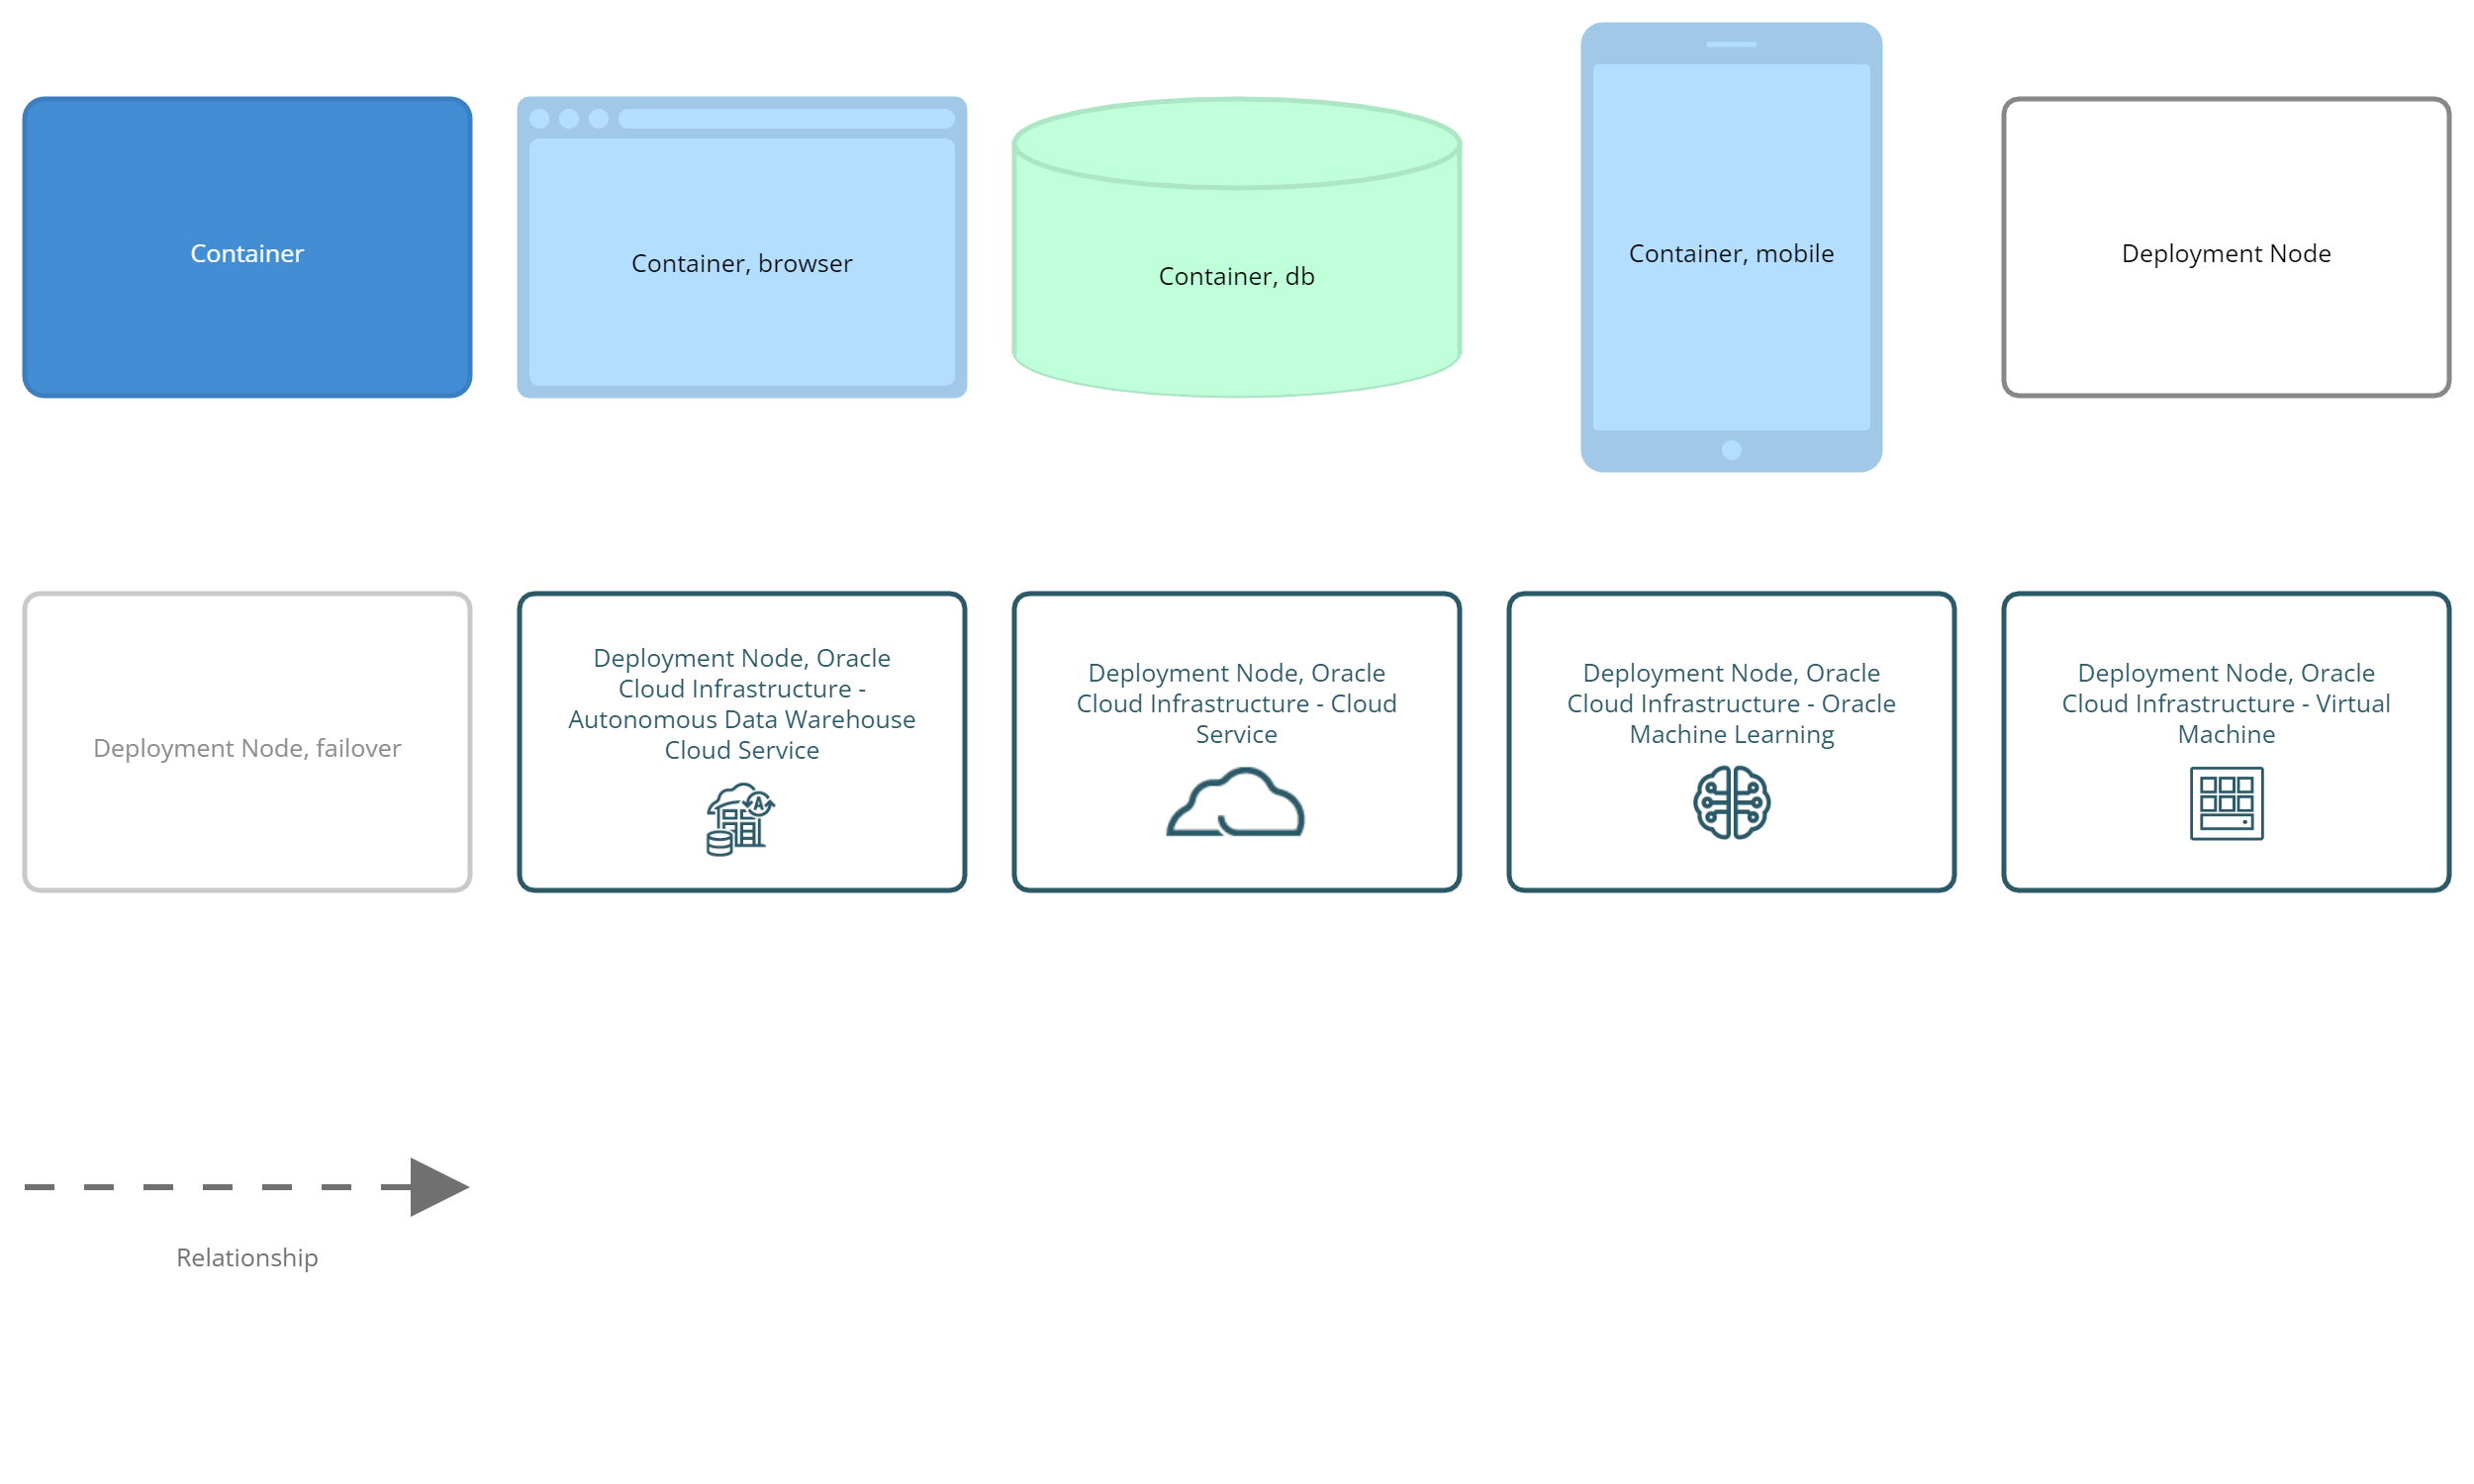
\includegraphics[trim=22 210 22 24,clip,width=0.95\paperwidth]{images/c4/deployment_diagram-key.png}
    \end{adjustwidth}
    \caption{Deployment diagram key.}
    \label{fig:c4_deployment_key}
\end{figure}

\subsection{Delivering Architecturally Significant Requirements}
In section \ref{sec:storeReq}, four ASRs were identified for the Sahara eCommerce system.
These were the abililty to continue shopping on different devices, scalability, robustness and availability.

Implementing shared logic on an application server, as shown in figure \ref{fig:c4_deployment},
enables the web and mobile applications to share common logic and state.
This delivers the functionality of allowing a customer to start shopping on one device and to continue on another device.
It also minimises duplication of logic, as it is shared by the frontend applications.

Using separate computing infrastructure for the web server, application server, application database, and data mining service,
as shown in figure \ref{fig:c4_deployment}, provides more options to deliver scalability, robustness and availability.
For scalability and performance, each computing environment can be optimised for the services it delivers.
It also means that new infrastructure can be deployed to target specific bottlenecks.

\noindent
The system follows the \link{\emph{stateless architecture} pattern}{https://www.redhat.com/en/topics/cloud-native-apps/stateful-vs-stateless}.
The web and mobile applications do not store any application state (e.g. products currently stored in the shopping cart).
Every time the customer performs a transaction (e.g. viewing product details or adding a product to their shopping cart),
the web or mobile application sends a message to the application server to perform the action.
The application server then saves or loads data to or from the application database.

This means that web and mobile applications can send messages to a different application server for each request.
This facilitates scalability, robustness and availability.
A new application server can be started to cater for increasing system load, or to replace a failed server.
The stateless nature of the application server logic means that no data will be lost if a server fails,
or if a frontend application accesses a different application server in the middle of a customer's shopping experience.

Having multiple application servers, web servers, and multiple application databases,
means that if one server fails its load can be picked up by other servers.
Automating the process of starting or restarting servers improves robustness and availability.
Running the data mining service on Oracle's cloud infrastructure means that we can rely
on their management of services to guarantee our required level of scalability and availability.

One challenge of a stateless architecture is providing a replicated database that contains up-to-date copies of the system's state.
We will look at this issue later in the course.

By designing the architecture as a set of components running on different servers, it is also easier to migrate the application to cloud-based infrastructure.
Figure \ref{fig:c4_deployment} does not constrain the system to run on physical hardware hosted by Sahara eCommerce.
Any of the nodes could be provisioned by a service offered by a cloud provider.


\section{Tools}
We will use C4 as our standard notation in this course,
supplemented with UML diagrams when their level of detail is appropriate.
C4 is popular because it has a basic structure, but the rules are intentionally loose to make it easy to adopt.
You should use tools to aid the creation of your diagrams and documentation.

The important thing is that you should use a modelling tool, not a drawing tool.
A few drawing tools provide C4 templates.
The issue with drawing tools is that they do not know what the elements of the diagram mean.
If a container name is changed in a drawing tool, you will need to manually change it wherever it is referenced in other diagrams.
A modelling tool will track the information that describes the model, so that a change to a model element in one place,
will be replicated wherever that element appears in other diagrams.

There are a few tools that support C4. Some to consider are \link{Structurizr}{https://www.structurizr.com/},
\link{C4-PlantUML}{https://github.com/plantuml-stdlib/C4-PlantUML}, \link{Archi}{https://www.archimatetool.com/},
\link{IcePanel}{https://icepanel.io/}, or \link{Gaphor}{https://gaphor.org/}.

\begin{description}
    \item[Structurizr]
        was developed by Simon Brown as a tool to support generating C4 diagrams from textual descriptions.
        UQ students may register for free access to the paid version of the \link{Structurizr Cloud Service}{https://structurizr.com/help/academic}.
        You must use your \texttt{student.uq.edu.au} or \texttt{uq.net.au} email address when you register to get free access.
        Structurizr is an \link{open source tool}{https://github.com/structurizr/}.
        You can use a \link{domain specific language}{https://docs.structurizr.com/dsl/language} to describe a C4 model,
        or you can embed the details in \link{Java}{https://docs.structurizr.com/java} code.
    \item[C4-PlantUML] extends the UML modelling tool PlantUML to support C4.
    \item[Archi] is an open source visual modelling tool that
        \link{supports C4}{https://www.archimatetool.com/blog/2020/04/18/c4-model-architecture-viewpoint-and-archi-4-7/} and ArchiMate models.
    \item[IcePanel] is a cloud-based visual modelling tool that supports C4. There is a limited free license for the tool.
    \item[Gaphor] is an open source visual modelling tool that supports UML and C4.
\end{description}

\subsection{Textual vs Visual Modelling}
The tools described above include both graphical and textual modelling tools.
Graphical tools, such as Archi and Gaphor, allow you to create models by drawing them.
This approach is often preferred by \link{visually oriented learners}{https://vark-learn.com/strategies/visual-strategies/}.
Text-based tools, such as C4-PlantUML and Structurizr, allow you to create models by providing a textual description of the model.
This approach is often preferred by \link{read/write oriented learners}{https://vark-learn.com/strategies/readwrite-strategies/}.

Despite preferences, there are situations where there are advantages of using a text-based modelling tool.
Being text, the model can be stored and versioned in a version control system (e.g. git).
For team projects, it is much easier for everyone to edit the model and ensure that you do not destroy other team members' work.
It is also possible to build a tool pipeline that will generate diagrams and embed them into the project documentation.

Text-based modelling tools, such as Structurizr or C4-PlantUML, use a
\link{domain specific language}{https://opensource.com/article/20/2/domain-specific-languages} (DSL) to describe the model.
These tools require that you learn the syntax and semantics of the DSL.
The following sources of information will help you learn the Structurizr DSL:
\begin{itemize}[nosep]
    \item \link{language reference manual}{https://docs.structurizr.com/dsl/language},
    \item \link{language examples}{https://docs.structurizr.com/dsl/cookbook/}, 
    \item \link{on-line editable examples}{https://structurizr.com/dsl}, and
    \item \link{off-line tool}{https://github.com/structurizr/cli}.
\end{itemize}

\subsection{Example Diagrams}
You may find the Sahara eCommerce C4 model useful as an example of a number of features of the Structurizr DSL.
You are able to download the C4 model of the Sahara eCommerce example, from the course website.
The \link{C4 model}{https://csse6400.uqcloud.net/resources/c4_model.zip}
was created using the \link{Structurizr}{https://www.structurizr.com/} DSL.



\section{\textit{Software Architecture in Practice} Views}
The seminal architecture book, \textit{Software Architecture in Practice} \cite{bass2021software},
categorises architectural views into three groups.
These three groups each answer different questions about the architecture, specifically:
\begin{description}
    \item[Module Views] How implementation components of a system are structured and depended upon.
    \item[Component-and-connector Views] How individual components communicate with each other.
    \item[Allocation Views] How the components are allocated to personnel, file stores, hardware, etc.
\end{description}

\subsection{Module Views}
Module views are composed of modules, which are static units of functionality such as classes, functions, packages, or whole programs.
The defining characteristic of a module is that it represents software responsible for some well-defined functionality.
For example, a class which converts JSON to XML would be considered a module, as would a function which performs the same task.

The primary function of module views is to communicate the dependencies of a module.
Rarely does software work completely in isolation, often it is constructed with implicit or explicit dependencies.
A module which converts JSON to XML might depend upon a module which parses JSON and a module which can format XML.
Module views make these dependencies explicit.

Module views focus on the developer's perspective of how the software is implemented, rather than how it manifests itself when deployed in a computing environment.

\begin{figure}[ht]
\centering
\begin{subfigure}[b]{\textwidth}
\begin{shaded}
\begin{lstlisting}[style=python]
import json
import xml

class JSONtoXML:
    def load(self, json_file):
        with open(json_file) as f:
            data = json.load(f)
        self.data = self.convert(data)

    def export(self, xml_file):
        xml.write(xml_file, data)

    def convert(self, data: JSON) -> XML:
        ...
\end{lstlisting}
\end{shaded}
\caption{Pseudo-code to convert JSON to XML}
\end{subfigure}


\begin{subfigure}[b]{\textwidth}
\begin{center}
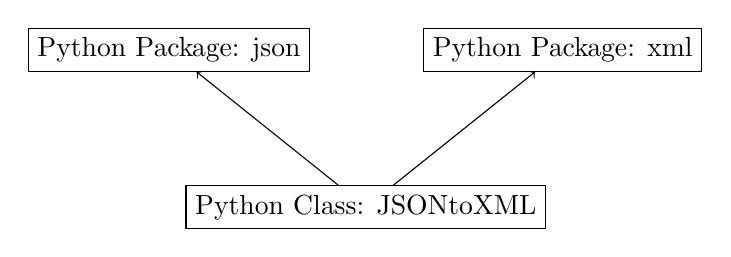
\begin{tikzpicture}
    \node[draw] (json) at (0,0) {Python Package: json};
    \node[draw] (xml) at (5,0) {Python Package: xml};
    \node[draw] (jsontoxml) at (2.5,-2) {Python Class: JSONtoXML};

    \path [->] (jsontoxml) edge node {} (json);
    \path [->] (jsontoxml) edge node {} (xml);
\end{tikzpicture}
\end{center}
\caption{An example of a module view which illustrates the dependencies of the \texttt{JSONtoXML} class}
\end{subfigure}
\caption{A simple module view of a JSON to XML program.}
\end{figure}

\subsection{Component-and-Connector Views}
Component-and-connector views focus on the structures that deliver the runtime, or dynamic behaviour of a system.
Components are units which perform some computation or operation at runtime.
These components could overlap with the modules of a module view but are often at a higher level of abstraction.
The focus of component-and-connector views is how these components communicate at runtime.
Runtime communication is the connector of components.
For example, a service which registers users to a website might have new registrations communicated via a REST request.
The service may then communicate the new user information to a database via SQL queries.

\noindent
When we look at software architecture, component-and-connector views are the most commonly used views.
They are common because they contain runtime information which is not easily automatically extracted.
Module views can be generated after the fact, i.e. it is easy enough for a project to generate a UML class diagram.
(Simple tools will create an unreadably complex class diagram.
Tagging important information in the source code, or manually removing small details is required to end up with readable diagrams.)
Component-and-connector views are often maintained manually by architects and developers.

\subsection{Allocation Views}
According to Bass et al, allocation views map the software's structures to the system's non-software structures \cite{bass2021software}.
They include concepts such as who is developing which software elements,
where are source files stored for different activities such as development and testing,
and where are software elements executed.
The first two points are important for project management and build management.
The last point of how the software is executed on different processing nodes is important for architectural design.
This is sometimes called the \emph{deployment structure} or the software system's \emph{physical architecture}.

Understanding the physical architecture (simplistically the hardware\footnote{Whether it is virtualised or physical hardware}
on which the software is executed) is important when designing the software's \emph{logical architecture}.
Component-and-connector views describe the software's logical architecture.
This design of the logical architecture must contain components that can be allocated appropriately to processing nodes,
and these nodes must have communication links that enable the components to interact.


\section{4+1 Views}
Philippe Kruchten was one of the earliest to advocate the idea of using views to design and document software architectures.
In ``4+1 View Model of Software Architecture'' \cite{4+1-model} he describes five different views.
These are logical, process, development, physical, and scenario views, which are summarised below.
\begin{description}
    \item[Logical] How functionality is implemented, using class and state diagrams.
    \item[Process] Runtime behaviour, including concurrency, distribution, performance and scalability.
                            Sequence, communication and activity diagrams are used to describe this view.
    \item[Development] The software structure from a developer's perspective, using package and component diagrams.
                                    This is also known as the implementation view.
    \item[Physical] The hardware environment and deployment of software components.
                            This is also known as the deployment view.
    \item[Scenario] The key usage scenarios that demonstrate how the architecture delivers the functional requirements.
                             This is the `+1' view as it is used to validate the software architecture.
                             This is also known as the use case view, as high-level use case diagrams are used to outline the key use cases and actors.
							 A high-level use case diagram provides contextual information, similar to the intent of the C4 context diagram.
							 A use case diagram allows more information to be conveyed and if it is supported with activity diagrams,
							 it provides a significant amount of information that can be used to validate the architecture.
\end{description}
The experience which led to the development the 4+1 View Model was developing the air traffic control management system for Canada.
The system provides an integrated air traffic control system for the entire Canadian airspace.
This airspace is about double the size of the Australian airspace and borders the two busiest airspaces in the world.
The project's architecture was designed by a team of three people led by Philippe.
Development was done by a team of 2500 developers from two large consulting companies.
The project was delivered on-time and on-budget, with three incremental releases in less than three years\footnote{Contrast
this to the United States Federal Aviation Administration's Advanced Automation System project from a similar era.
The original estimate was \$2.5 billion and fourteen years to implement.
The project was effectively cancelled after twelve years.
By then the estimate had almost tripled and the project was at least a decade behind schedule \cite{faa-aas}.}.
This project also developed many of the ideas that led to the Rational Unified Process \cite{kruchten2004rational}.


\section{Conclusion}
Architectural views help developers understand different dimensions and details of a complex software architecture.
They are useful both during design and as documentation.
During design, views help you to focus on a particular aspect of the software architecture and ensure that it will allow the system to deliver all of its requirements.
As documentation, views help developers to understand how different aspects of the architecture are intended to behave.

We have intentionally looked at a few different approaches to helping you describe a software architecture.
You should be conversant with multiple different approaches.
The hallmark of a professional is to know when to select a particular approach.

If you compare the ``4+1 View Model'' \cite{4+1-model} with the views described in \textit{Software Architecture in Practice} (SAP) \cite{bass2021software},
you will see that there are obvious similarities but also some differences.
The logical, development and process views from the 4+1 view model map closely to the module and component-and-connector (C\&C) views from SAP.
The physical view corresponds to the allocation view.
The 4+1 view model also includes the scenario view, which does not correspond directly to the SAP views.

The scenario view is used to demonstrate how the architecture described in the other views delivers the core functional requirements.
It is used while designing a software architecture to validate that it is suitable for the system.

Kruchten intentionally separated the process view from the logical and development views,
rather than bundling them together like the C\&C view in SAP.
This is because for some systems the dynamic details, which are described by the process view, can be complex and important.
Dealing with issues such as complex concurrency, real-time interactions or latency, can often be more easily considered by having a separate view for them.

Kruchten's experience with Canada's integrated, nation-wide, air traffic control system was such a case.
Data from radar systems and aircraft transponders have to be processed and reported to air traffic controllers in near real-time.
With thousands of input sources and hundreds of controller stations, understanding concurrency issues is critical.
Tracking aircraft from one control space to another means that communication latency is important.
Each control space has its own hardware and is separated from neighbouring spaces by hundreds or thousands of kilometres.

The C4 model does not explicitly include the concept of views.
Like SAP, it emphasises the structure of the software architecture, adding a hierarchical lens in its structural view.
These diagrams map to the 4+1 logical and development views and the SAP module and C\&C views.
Its behavioural view maps to aspects of the 4+1 process view.
Its infrastructure view maps to the 4+1 physical view and the SAP allocation view.

As a software architect you need to choose which views provide meaningful information about your software system.
The graphical notation used to describe a view is only one part of the view (though an important part).
Ensure you provide enough supporting information so others will know how to work with your architecture and why you made the choices that you did.